\newcommand{\hopac}{Hopac}
\chapter{\label{chap:median}Statistical Operations and Median Filtering in \glsfmtname{cps}}

Many computer vision and image processing operations have some potential for parallelism.  Indeed, a number of them can be regarded as \emph{embarrassingly parallel}.  That is, the process involves a considerable number of independent sub-process steps, and so those steps may safely be performed concurrently.  Some of those algorithms either are explicitly characterised in terms of message passing, such as \gls{sm} with \gls{bp} \cite{Liang2011} or semi-global matching \cite{Drory2014}, or could potentially be viewed as such, \eg{} \glspl{mwt} applied to images.

\Gls{medianfilter}ing \cite[Chap. 3.4.1]{Gimelfarb2018}, \cite{Fisher2016} is a \gls{mwt} operation in image processing used to remove random `salt \& pepper' noise from images.  Such noise is characterised by pixel colouration values at the extreme high and low ends of the range of possible values.  At its simplest, \gls{medianfilter}ing recovers an approximation of the non-noisy image by taking the median of all pixel values in a window around each pixel and creating a new image using said median values for the pixels.

Finding the median of a multiset is a well-known fundamental statistical operation.  Likely the way that many people were first taught to perform it was to sort the relevant multiset, count the relevant multiset, halve the count, and then take the number at that position in the multiset.  All of these operations individually, and other similar ones, are relatively simple in \gls{cps} when working with numeric terms (\ie{} terms holding multiplicities of the unary digit \(\cpundig\)).  Moreover, it is also simple to combine these operations into one overarching \gls{ruleset} to carry out the requisite process.

% This \namecref{chap:median} seeks to model \gls{medianfilter}ing using \gls{cps}, as another test of the power and versatility of \gls{cps}, a more intensive test of the utility of \gls{cml} for \gls{cps}, and to explore whether using \gls{cml} -- as a method of structuring computations around message passing -- could be beneficial when applied to a \gls{mwt}, using the \gls{medianfilter} as its particular example.  It starts by describing how to perform a variety of fundamental statistical operations with \gls{cps}, going from less complex to more complex, and re-using earlier ones as part of the implementation of later ones.  This builds up to performing selection -- taking the \(n^{\text{th}}\) element of a sorted multiset -- which can be used to implement the median operation.

This \namecref{chap:median} seeks to model \gls{medianfilter}ing using \gls{cps}, as:
\begin{inparaenum}[a)]
\item  another test of the power and versatility of \gls{cps};
\item a more intensive test of the utility of \gls{cml} for \gls{cps}; and,
\item to explore whether using \gls{cml} as a method of structuring computations around message passing could be beneficial when applied to a \gls{mwt}.
\end{inparaenum}
% using the \gls{medianfilter} as its particular example.
It starts by describing how to perform various fundamental statistical operations with \gls{cps}, going from less complex to more complex, and re-using earlier ones as part of later ones.  This builds up to performing selection -- taking the \(n^{\text{th}}\) element of a sorted multiset -- which can be used to implement the median operation.

Before moving to the \gls{cps} \gls{medianfilter} solution, several earlier works on applying \gls{mc} to image processing are summarised, providing background and context on this effort, though the current \namecref{chap:median} is the first known application of \gls{mc} directly to the \gls{medianfilter}.  Next, this \namecref{chap:median} demonstrates the combination of selection and counting to find the median of a multiset, with antiport message passing between pixels used to build up the multisets in each pixel.  Finally, three different practical implementations of \gls{medianfilter}ing are introduced and assessed.  The first implementation is a simple naïve approach, as many programmers might write; the second is a \gls{cml} one very closely connected to the \gls{cps} solution; while the third sits conceptually somewhere between the two and is based on work by \citeauthor{Braunl2001} \cite{Braunl2001}.  The focus in this final \namecref{sec:median:cpsmedianfilter} is on examining the potential benefit of using a different principle to structure the processing, as much as it is on the achieved image results.
%-----------------------------------------------------------------------------------
\section{Statistical Operations}\label{sec:median:stats}
%-----------------------------------------------------------------------------------

This section presents and discusses procedures in \gls{cps} for the following fundamental statistical operations on numerical sets and multisets:
\begin{itemize}
    \item Finding the minimum and maximum elements
    \item Determining the overall number and counting the frequency of elements
    \item Computing the sum, mean, and mode over all elements
    \item Sorting elements
    \item Selecting the \(n^{\text{th}}\) (and thus median) element
\end{itemize}

Leveraging the power of \gls{cps} -- logical pattern matching on associative data objects -- \emph{all} of the presented procedures run in constant time \bigoh{1} and require small, fixed \glspl{ruleset} for all cases.  For brevity, these rules consider only the case of non-empty (multi)sets of natural numbers greater than zero (\(\mathbb{N}^+\)), and their total order (\(\leq\)).  Extensions to handle zero values and empty sets are not complicated, but would inflate \glspl{ruleset} by a few additional rules without adding significant value (although they would not alter the time complexity).

At the start (``step 0'') of each presented operation, assume an arbitrary non-empty set or multiset of \(s\) objects, which each hold an arbitrary number.  For each example with a set, the starting \(s\) terms assumed present are:  \[S_1 = \cpset{\cpfunc{s}{2}, \cpfunc{s}{3}, \cpfunc{s}{5}, \cpfunc{s}{6}, \cpfunc{s}{7}}\]  Likewise, the assumed multiset is \[S_2 = \cpset{\cpfunc{s}{2}, \cpfunc{s}{2}, \cpfunc{s}{3}, \cpfunc{s}{5}, \cpfunc{s}{5}, \cpfunc{s}{6}, \cpfunc{s}{6}, \cpfunc{s}{6}, \cpfunc{s}{7}}\]  In almost all cases, the operations apply equally to sets and multisets, so the examples assume the presence of \(S_2\) inside the \gls{tlc}.  The exceptions to that are in \cref{sec:median:sortsets} and \cref{sec:median:selectsets}, where \(S_1\) is assumed instead, and \cref{sec:median:sortmultisetid} and \cref{sec:median:sortmultisetid}, which use \(S_2\) with an additional datum for each element.  The rules provided are all non-destructive with respect to the multiset \(S\).  Destructive versions are simple to derive from the non-destructive ones, so are omitted.

In all cases, the rules are written so that the final result is found in one or more \(r\) \gls{functor} objects, as appropriate.  Examples of the evolution are given in tabular form immediately after the rules for each operation.  Modified objects are presented with their outermost \gls{functor} in boldface, \eg{} \(\cpfunc{r}{0}\) to \(\mathbf{\cpfunc{r}{4}}\).  Deleted objects are struck out, \eg{} \(\cpfunc{r'}{2}\) to \sout{\(\cpfunc{r'}{2}\)}, and omitted entirely from later steps.

%%%%%%%%%%%%%%%%%%

%-------------------------------------------------------
\subsection{\label{sec:median:minmax}Minimum and Maximum}
%-------------------------------------------------------

The below states the rules and steps necessary to find the minimum and maximum of a multiset.  A more comprehensive discussion (from which the following are derived) of these operations can be found in \cite{Cooper2019,Nicolescu2018}.

%-----------------------------------------
\subsubsection{Minimum --- \bigoh{1}}\label{sec:median:min}
%-----------------------------------------

\begin{proposition}\label{prop:median:min}
Finding the minimum of a multiset takes one step.
\end{proposition}

\begin{proof}
Consider \cref{rules:median:min} and the example in \cref{tab:median:min}.  The rule to find the minimum selects an \(s\) term's value, such that there is no other \(s\) with a strictly lower value.
\end{proof}

\begin{cprulesetfloat}
\begin{cpruleset}
\cprule*{s_1}{}{\cponce}{s_2}{\cpfunc{r}{R\cpundig T}}
\cppromoter{\cpfunc{s}{R\cpundig T}}
\cpinhibitor{\cpfunc{s}{R}}
\end{cpruleset}
\caption{\label{rules:median:min}\Gls{ruleset} to find the minimum element in a multiset}
\end{cprulesetfloat}

\begin{table}[htbp]
\centering
\begin{tabular}{|r|l|}
    \hline
    \textbf{Step} & \textbf{New, Modified \& Deleted Objects} \\ \hline
    1 & \(\cpfunc{r}{2}\) \\ \hline
\end{tabular}
\caption[Example evolution of \cref{rules:median:min} to find the minimum element in a multiset]{\label{tab:median:min}Example evolution of \cref{rules:median:min} starting on multiset \(S_2\)}
\end{table}

%-----------------------------------------
\subsubsection{\label{sec:median:max}Maximum --- \bigoh{1}}
%-----------------------------------------

\begin{proposition}\label{prop:median:max}
Finding the maximum of a multiset takes one step.
\end{proposition}

\begin{proof}
Consider \cref{rules:median:max} and the example in \cref{tab:median:max}.  The rule to find the maximum selects an \(s\) term's value, such that there is no other \(s\) with a strictly higher value.
\end{proof}

\begin{cprulesetfloat}
\begin{cpruleset}

\cprule*{s_1}{}{\cponce}{s_2}{\cpfunc{r}{R}}
\cppromoter{\cpfunc{s}{R}}
\cpinhibitor{\cpfunc{s}{R\cpundig \_}}

\end{cpruleset}
\caption{\label{rules:median:max}\Gls{ruleset} to find the maximum element in a multiset}
\end{cprulesetfloat}

\begin{table}[htbp]
\centering
\begin{tabular}{|r|l|}
    \hline
    \textbf{Step} & \textbf{New, Modified \& Deleted Objects} \\ \hline
    1 & \(\cpfunc{r}{7}\)\\ \hline
\end{tabular} 
\caption[Example evolution of \cref{rules:median:max} to find the maximum element in a multiset]{\label{tab:median:max}Example evolution of \cref{rules:median:max} starting on multiset \(S_2\)}
\end{table}

%%%%%%%%%%%%%%%%%%

%-------------------------------------------------------
\subsection{Counting}\label{sec:median:counting}
%-------------------------------------------------------

%-----------------------------------------
\subsubsection{Counting Elements --- \bigoh{1}}\label{sec:median:countelems}
%-----------------------------------------

\begin{proposition}\label{prop:median:countelems}
Determining the magnitude of a multiset takes two steps.
\end{proposition}

\begin{proof}
Consider \cref{rules:median:countelems} and the example in \cref{tab:median:countelems}.  \cpRuleref{rules:median:countelems:1} creates an empty term to store the result, and then \cpruleref{rules:median:countelems:2} tallies the elements present.
\end{proof}

\begin{cprulesetfloat} \begin{cpruleset}

\cprule[rules:median:countelems:1]{s_1}{}{\cponce}{s_2}{\cpfunc{r}{\cpempty}}

\cprule[rules:median:countelems:2]{s_2}{\cpfuncms{r}{\,}}{\cpmaxpar}{s_3}{\cpfuncms{r}{\cpundig}}
\cppromoter{\cpfunc{s}{\_}}

\end{cpruleset}
\caption{\label{rules:median:countelems}\Gls{ruleset} to find the magnitude of a multiset}
\end{cprulesetfloat}

\begin{table}[htbp]
\centering
   \begin{tabular}{|r|l|}
    \hline
    \textbf{Step} & \textbf{New, Modified \& Deleted Objects} \\ \hline
    1 & \(\cpfunc{r}{0}\)\\ \hline
    
    2 & \(\mathbf{\cpfunc{r}{9}}\)\\ \hline
\end{tabular}
\caption[Example evolution of \cref{rules:median:countelems} to find the magnitude of a multiset]{\label{tab:median:countelems}Example evolution of \cref{rules:median:countelems} starting on multiset \(S_2\)}
\end{table}

%-----------------------------------------
\subsubsection{Counting Frequency of Elements --- \bigoh{1}}\label{sec:median:countfreq}
%-----------------------------------------

\begin{proposition}\label{prop:median:countfreq}
Counting the occurrence -- essentially creating a histogram -- of the values in a multiset takes three steps.
\end{proposition}

\begin{proof}
Consider \cref{rules:median:countfreq} and the example in \cref{tab:median:countfreq}.  \cpRuleref{rules:median:countfreq:1} creates a tally \(r\) term for every \(s\) term, while \cpruleref{rules:median:countfreq:2} eliminates any ensuing duplicates, leaving only one \(r\) per unique value stored in any \(s\).  Lastly, \cpruleref{rules:median:countfreq:3} performs a similar operation to \cref{sec:median:countelems}, incrementing each \(r\) term's tally by one for each \(s\) term containing the corresponding value.
\end{proof}

\begin{cprulesetfloat}
\begin{cpruleset}
\cprule[rules:median:countfreq:1]{s_1}{}{\cpmaxpar}{s_2}{\cpfuncn{r}{R}{\cpempty}}
\cppromoter{\cpfunc{s}{R}}

\cprule[rules:median:countfreq:2]{s_2}{\cpfuncn{r}{R}{\_}}{\cpmaxpar}{s_3}{}
\cppromoter{\cpfuncn{r}{R}{\_}}

\cprule[rules:median:countfreq:3]{s_3}{\cpfuncnms{r}{R}{\,}}{\cpmaxpar}{s_4}{\cpfuncnms{r}{R}{\cpundig}}
\cppromoter{\cpfunc{s}{R}}
\end{cpruleset}
\caption{\label{rules:median:countfreq}\Gls{ruleset} to count the occurrence frequency of elements in a multiset}
\end{cprulesetfloat}

\begin{table}[htbp]
\centering
   \begin{tabular}{|r|l|}
    \hline
    \textbf{Step} & \textbf{New, Modified \& Deleted Objects} \\ \hline
    1 & \(\cpfuncn{r}{2}{0}\), \(\cpfuncn{r}{2}{0}\), \(\cpfuncn{r}{3}{0}\), \(\cpfuncn{r}{5}{0}\), \(\cpfuncn{r}{5}{0}\), \(\cpfuncn{r}{6}{0}\), \(\cpfuncn{r}{6}{0}\), \(\cpfuncn{r}{6}{0}\), \(\cpfuncn{r}{7}{0}\)\\ \hline
    
    2 & \(\cpfuncn{r}{2}{0}\), \sout{\(\cpfuncn{r}{2}{0}\)}, \(\cpfuncn{r}{3}{0}\), \(\cpfuncn{r}{5}{0}\), \sout{\(\cpfuncn{r}{5}{0}\)}, \(\cpfuncn{r}{6}{0}\), \sout{\(\cpfuncn{r}{6}{0}\)}, \sout{\(\cpfuncn{r}{6}{0}\)}, \(\cpfuncn{r}{7}{0}\)\\ \hline
    
    3 & \(\mathbf{\cpfuncn{r}{2}{2}}\), \(\mathbf{\cpfuncn{r}{3}{1}}\), \(\mathbf{\cpfuncn{r}{5}{2}}\), \(\mathbf{\cpfuncn{r}{6}{3}}\), \(\mathbf{\cpfuncn{r}{7}{1}}\)\\ \hline
\end{tabular}
\caption[Example evolution of \cref{rules:median:countfreq} to count the occurrence frequency of elements in a multiset]{\label{tab:median:countfreq}Example evolution of \cref{rules:median:countfreq} starting on multiset \(S_2\)}
\end{table}

\Cref{rules:median:countfreq} works equally well for sets, but the frequency of each element present will be one due to the nature of a set.

%-------------------------------------------------------
\subsection{Sum, Mean and Mode}\label{sec:median:sumeanmode}
%-------------------------------------------------------

%-----------------------------------------
\subsubsection{Sum --- \bigoh{1}}\label{sec:median:sum}
%-----------------------------------------

\begin{proposition}\label{prop:median:sum}
Computing the sum of the elements in a multiset requires two steps.
\end{proposition}

\begin{proof}
Consider \cref{rules:median:sum} and the example in \cref{tab:median:sum}.  These rules act very similarly to \cref{sec:median:countelems}, but add the total stored value in every \(s\) term to the \(r\) term, rather than simply one \(\cpundig\) per \(s\) term.
\end{proof}

\begin{cprulesetfloat} \begin{cpruleset}
\cprule{s_1}{}{\cponce}{s_2}{\cpfunc{r}{\cpempty}}
\cprule{s_2}{\cpfuncms{r}{\,}}{\cpmaxpar}{s_3}{\cpfuncms{r}{R}}
\cppromoter{\cpfunc{s}{R}}
\end{cpruleset}
\caption{\label{rules:median:sum}\Gls{ruleset} to find the sum of numeric elements in a multiset}
\end{cprulesetfloat}

\begin{table}[htbp]
\centering
   \begin{tabular}{|r|l|}
    \hline
    \textbf{Step} & \textbf{New, Modified \& Deleted Objects} \\ \hline
    1 & \(\cpfunc{r}{0}\)\\ \hline
    2 & \(\cpfunc{r}{42}\)\\ \hline

\end{tabular}
\caption[Example evolution of \cref{rules:median:sum} to find the sum of numeric elements in a multiset]{\label{tab:median:sum}Example evolution of \cref{rules:median:sum} starting on multiset \(S_2\)}
\end{table}

%-----------------------------------------
\subsubsection{Mean --- \bigoh{1}}\label{sec:median:mean}
%-----------------------------------------

\begin{proposition}\label{prop:median:mean}
Finding the (whole number) mean of a multiset requires four steps.
\end{proposition}

\begin{proof}
Consider \cref{rules:median:mean} and the example in \cref{tab:median:mean}.  Computing the mean is mostly a combination of two previous operations:  Sum the elements (\cref{sec:median:sum}), and divide by the count of elements (\cref{sec:median:countelems}).  The summing and counting may be performed simultaneously in two steps, with two extra steps for the division.
\end{proof}

\begin{cprulesetfloat}
\begin{cpruleset}
\cprule{s_1}{}{\cponce}{s_2}{\cpfunc{c}{\cpempty} \; \cpfunc{r}{\cpempty} \; \cpfunc{r'}{\cpempty}}

\cprule{s_2}{\cpfuncms{c}{\,}}{\cpmaxpar}{s_3}{\cpfuncms{c}{\cpundig}}
\cppromoter{\cpfunc{s}{\_}}

\cprule{s_2}{\cpfuncms{r}{\,} \; \cpfuncms{r'}{\,}}{\cpmaxpar}{s_3}{\cpfuncms{r}{R} \; \cpfuncms{r'}{R}}
\cppromoter{\cpfunc{s}{R}}

\cprule[rules:median:mean:4]{s_3}{\cpfuncms{r}{C} \; \cpfuncms{r'}{C}}{\cpmaxpar}{s_4}{\cpfuncms{r}{\cpundig} \; \cpfuncms{r'}{\,}}
\cppromoter{\cpfunc{c}{C}}

\cprule[rules:median:mean:5]{s_4}{\cpfunc{r}{QR} \; \cpfunc{r'}{R}}{\cponce}{s_5}{\cpfunc{r}{Q}}
\end{cpruleset}
\caption{\label{rules:median:mean}\Gls{ruleset} to find the mean of elements in a multiset}
\end{cprulesetfloat}

\begin{table}[htbp]
\centering
  \begin{tabular}{|r|l|}
    \hline
    \textbf{Step} & \textbf{New, Modified \& Deleted Objects} \\ \hline
    1 & \(\cpfunc{c}{0}\), \(\cpfunc{r}{0}\), \(\cpfunc{r'}{0}\)\\ \hline
    2 & \(\mathbf{\cpfunc{c}{9}}\), \(\mathbf{\cpfunc{r}{42}}\), \(\mathbf{\cpfunc{r'}{42}}\)\\ \hline
    3 & \(\mathbf{\cpfunc{r}{11}}\), \(\mathbf{\cpfunc{r'}{6}}\)\\ \hline
    4 & \(\mathbf{\cpfunc{r}{5}}\), \sout{\(\cpfunc{r'}{6}\)}\\ \hline

\end{tabular}
\caption[Example evolution of \cref{rules:median:mean} to find the mean of elements in a multiset]{\label{tab:median:mean}Example evolution of \cref{rules:median:mean} starting on multiset \(S_2\)}
\end{table}

Rules \cpruleref*{rules:median:mean:4} and \cpruleref*{rules:median:mean:5} perform ceiling integer division.  \cpRuleref{rules:median:mean:4} removes \(C\) copies of the unary digit from \(r\) and adds one copy back to it.  This is repeated as many times as possible, given the number of digits available.  What is left in \(r\) at the end of the step is, in effect, the quotient plus the remainder.  In this example, with a count of nine and a sum of forty-two, the removal can be applied four times, for a total of thirty-six unary digits removed.  Five more are added at the end of the step, meaning a total of eleven remains.  This is not the correct result of ceiling integer division but is the correct quotient (5) plus the remainder (6).  Thus, another copy of the total is kept and divided, without the quotient added back in.  This leaves \cpruleref{rules:median:mean:5} to compute the correct final result by deducting the remainder from the combined quotient and remainder.

%-----------------------------------------
\subsubsection{Mode --- \bigoh{1}}  \label{sec:median:mode}
%-----------------------------------------

\begin{proposition}\label{prop:median:mode}
Finding the mode of the elements in a multiset requires four steps.
\end{proposition}

\begin{proof}
Consider \cref{rules:median:mode} and the example in \cref{tab:median:mode}.  As with the mean, this process combines other operations:  Counting the frequency of elements (\cref{sec:median:countfreq}) takes three steps, then selecting the maximum (\cref{sec:median:max}) uses one extra step.  Unlike in \cref{sec:median:mean}, the aforementioned \glspl{ruleset} cannot be used concurrently to reduce the number of steps required because the maximum-finding rule may only fire once the frequency counting process has concluded.
\end{proof}

% \cpresetrulenumber
\begin{cprulesetfloat}
\begin{cpruleset}
\cprule{s_1}{}{\cpmaxpar}{s_2}{\cpfuncn{c}{C}{\cpempty}}
\cppromoter{\cpfunc{s}{C}}

\cprule{s_2}{\cpfuncn{c}{C}{\_}}{\cpmaxpar}{s_3}{}
\cppromoter{\cpfuncn{c}{C}{\_}}

\cprule{s_3}{\cpfuncnms{c}{C}{\,}}{\cpmaxpar}{s_4}{\cpfuncnms{c}{C}{\cpundig}}
\cppromoter{\cpfunc{s}{C}}

\cprule{s_4}{}{\cponce}{s_5}{\cpfunc{r}{C}}
\cppromoter{\cpfuncn{c}{C}{R}}
\cpinhibitor{\cpfuncn{c}{\_}{R\cpundig \_}}

\end{cpruleset}
\caption{\label{rules:median:mode}\Gls{ruleset} to find the mode of the elements in a multiset}
\end{cprulesetfloat}

\begin{table}[htbp]
\centering
   \begin{tabular}{|r|l|}
    \hline
    \textbf{Step} & \textbf{New, Modified \& Deleted Objects} \\ \hline
    1 & \(\cpfuncn{c}{2}{0}\), \(\cpfuncn{c}{2}{0}\), \(\cpfuncn{c}{3}{0}\), \(\cpfuncn{c}{5}{0}\), \(\cpfuncn{c}{5}{0}\), \(\cpfuncn{c}{6}{0}\), \(\cpfuncn{c}{6}{0}\), \(\cpfuncn{c}{6}{0}\), \(\cpfuncn{c}{7}{0}\)\\ \hline
    
    2 & \(\cpfuncn{c}{2}{0}\), \sout{\(\cpfuncn{c}{2}{0}\)}, \(\cpfuncn{c}{3}{0}\), \(\cpfuncn{c}{5}{0}\), \sout{\(\cpfuncn{c}{5}{0}\)}, \(\cpfuncn{c}{6}{0}\), \sout{\(\cpfuncn{c}{6}{0}\)}, \sout{\(\cpfuncn{c}{6}{0}\)}, \(\cpfuncn{c}{7}{0}\)\\ \hline
    
    3 & \(\mathbf{\cpfuncn{c}{2}{2}}\), \(\mathbf{\cpfuncn{c}{3}{3}}\), \(\mathbf{\cpfuncn{c}{5}{2}}\), \(\mathbf{\cpfuncn{c}{6}{3}}\), \(\mathbf{\cpfuncn{c}{7}{1}}\)\\ \hline
    
    4 & \(\cpfuncn{c}{2}{2}\), \(\cpfuncn{c}{3}{3}\), \(\cpfuncn{c}{5}{2}\), \(\cpfuncn{c}{6}{3}\), \(\cpfuncn{c}{7}{1}\), \(\cpfunc{r}{5}\)\\ \hline
    
\end{tabular}
\caption[Example evolution of \cref{rules:median:mode} to find the mode of the elements in a multiset]{\label{tab:median:mode}Example evolution of \cref{rules:median:mode} starting on multiset \(S_2\)}
\end{table}

%-------------------------------------------------------
\subsection{Sorting}\label{sec:median:sorting}
%-------------------------------------------------------

In the current context, sorting is defined as appropriately associating each datum/element in a multiset with an ordered index in the range \([1,n]\), where \(n\) is equal to the magnitude (count of elements) of the multiset.\footnote{This can easily be switched to \([0,n)\) if desired.}  At the end of the process, the values in the multiset shall be sorted in typical ascending numerical order by associating indices with them.

For example, in the context of \(S_2\), this will be 
\begin{align*}
    \text{Element:}& &2 &&2 &&3 &&5 &&5 &&6 &&6 &&6 &&7\\
    \text{Index:}&   &1 &&2 &&3 &&4 &&5 &&6 &&7 &&8 &&9\\
\end{align*}

\Cref{sec:median:sortsets} \& \cref{sec:median:sortmultisetid} associate each element with the index individually, while \cref{sec:median:sortmultisetrange} groups identical multiset elements into ranges spanning the correct indices.

%-----------------------------------------
\subsubsection{Sorting Sets --- \bigoh{1}}  \label{sec:median:sortsets}
%-----------------------------------------

\begin{proposition}\label{prop:median:sortsets}
Sorting sets requires two steps.
\end{proposition}

\begin{proof}
Consider \cref{rules:median:sortsets} and the example in \cref{tab:median:sortsets}.  The rules for sorting a set work similarly to those for counting the frequency of elements (\cref{sec:median:countfreq}).  Instead of counting the occurrence of a particular value, however, these rules count the occurrence of values strictly less than the current value.  In each instance, this number plus one is equal to the value's correct index in the total ordering, thus sorting the values.
\end{proof}

\begin{cprulesetfloat}
\begin{cpruleset}
\cprule{s_1}{}{\cpmaxpar}{s_2}{\cpfuncn{r}{R}{\cpundig}}
\cppromoter{\cpfunc{s}{R}}

\cprule{s_2}{\cpfuncnms{r}{Y}{\,}}{\cpmaxpar}{s_3}{\cpfuncnms{r}{Y}{\cpundig}}
\cppromoter{\cpfunc{s}{X}}
\cppromoter{X \subsetneq Y}
\end{cpruleset}
\caption{\label{rules:median:sortsets}\Gls{ruleset} to sort the elements in a set}
\end{cprulesetfloat}

\begin{table}[htbp]
\centering
   \begin{tabular}{|r|l|}
    \hline
    \textbf{Step} & \textbf{New, Modified \& Deleted Objects} \\ \hline
    1 & \(\cpfuncn{r}{2}{1}\), \(\cpfuncn{r}{3}{1}\), \(\cpfuncn{r}{5}{1}\), \(\cpfuncn{r}{6}{1}\), \(\cpfuncn{r}{7}{1}\)\\ \hline
    2 & \(\cpfuncn{r}{2}{1}\), \(\mathbf{\cpfuncn{r}{3}{2}}\), \(\mathbf{\cpfuncn{r}{5}{3}}\), \(\mathbf{\cpfuncn{r}{6}{4}}\), \(\mathbf{\cpfuncn{r}{7}{5}}\)\\ \hline

\end{tabular}
\caption[Example evolution of \cref{rules:median:sortsets} to sort the elements in a set]{\label{tab:median:sortsets}Example evolution of \cref{rules:median:sortsets} starting on set \(S_1\)}
\end{table}

%-----------------------------------------
\subsubsection{Sorting Multisets into Ranges --- \bigoh{1}}\label{sec:median:sortmultisetrange}
%-----------------------------------------

\begin{proposition}\label{prop:median:sortmultisetrange}
Sorting a multiset into ordered, indexed ranges requires four steps.
\end{proposition}

\begin{proof}
Consider \cref{rules:median:sortmultisetrange} and the example in \cref{tab:median:sortmultisetrange}.  In these rules, the last two numbers for each ending \(t\) object give a range of indices -- with inclusive lower bounds and exclusive upper bounds -- in which the \(s\) numbers of the multiset may be found once ordered.  It requires four steps and relies on the fact that elements of the same value in a multiset are indistinguishable, and thus can be ordered among themselves arbitrarily.

\end{proof}

\begin{cprulesetfloat}
\begin{cpruleset}
\cprule[rules:median:sortmultisetrange:1]{s_1}{}{\cpmaxpar}{s_2}{\cpfuncnn{r}{R}{\cpundig}{\cpundig}}
\cppromoter{\cpfunc{s}{R}}

\cprule{s_2}{\cpfuncnn{r}{R}{\_}{\_}}{\cpmaxpar}{s_3}{}
\cppromoter{\cpfuncnn{r}{R}{\_}{\_}}

\cprule[rules:median:sortmultisetrange:3]{s_3}{\cpfunc{r}{Y}\{\,\}\{\,\}}{\cpmaxpar}{s_4}{\cpfunc{r}{Y}\{\cpundig\}\{\cpundig\}}
\cppromoter{\cpfunc{s}{X}}
\cppromoter{X \subsetneq Y}

\cprule[rules:median:sortmultisetrange:4]{s_4}{\cpfuncnnms{r}{R}{X}{\,}}{\cpmaxpar}{s_5}{\cpfuncnnms{r}{R}{X}{\cpundig}}
\cppromoter{\cpfunc{s}{R}}

\end{cpruleset}
\caption{\label{rules:median:sortmultisetrange}\Gls{ruleset} to sort the elements of a multiset into indexed ranges}
\end{cprulesetfloat}

\begin{table}[htbp]
\centering
  \begin{tabular}{|r|l|}
    \hline
    \textbf{Step} & \textbf{New, Modified \& Deleted Objects} \\ \hline
    1 & \(\cpfuncnn{r}{2}{1}{1}\), \(\cpfuncnn{r}{2}{1}{1}\), \(\cpfuncnn{r}{3}{1}{1}\), \(\cpfuncnn{r}{5}{1}{1}\), \(\cpfuncnn{r}{5}{1}{1}\), \(\cpfuncnn{r}{6}{1}{1}\),\\& \(\cpfuncnn{r}{6}{1}{1}\), \(\cpfuncnn{r}{6}{1}{1}\), \(\cpfuncnn{r}{7}{1}{1}\)\\ \hline
    
    2 & \(\cpfuncnn{r}{2}{1}{1}\), \sout{\(\cpfuncnn{r}{2}{1}{1}\)}, \(\cpfuncnn{r}{3}{1}{1}\), \(\cpfuncnn{r}{5}{1}{1}\), \sout{\(\cpfuncnn{r}{5}{1}{1}\)}, \(\cpfuncnn{r}{6}{1}{1}\),\\& \sout{\(\cpfuncnn{r}{6}{1}{1}\)}, \sout{\(\cpfuncnn{r}{6}{1}{1}\)}, \(\cpfuncnn{r}{7}{1}{1}\)\\ \hline
    
    3 & \(\cpfuncnn{r}{2}{1}{1}\), \(\mathbf{\cpfuncnn{r}{3}{3}{3}}\), \(\mathbf{\cpfuncnn{r}{5}{4}{4}}\), \(\mathbf{\cpfuncnn{r}{6}{6}{6}}\), \(\mathbf{\cpfuncnn{r}{7}{9}{9}}\)\\ \hline
    
    4 & \(\mathbf{\cpfuncnn{r}{2}{1}{3}}\), \(\mathbf{\cpfuncnn{r}{3}{3}{4}}\), \(\mathbf{\cpfuncnn{r}{5}{4}{6}}\), \(\mathbf{\cpfuncnn{r}{6}{6}{9}}\), \(\mathbf{\cpfuncnn{r}{7}{9}{10}}\)\\ \hline
\end{tabular} 
\caption[Example evolution of \cref{rules:median:sortmultisetrange} to sort the elements of a multiset into indexed ranges]{\label{tab:median:sortmultisetrange}Example evolution of \cref{rules:median:sortmultisetrange} starting on multiset \(S_2\)}
\end{table}

In this example, 2s are in the index range \([1,3)\), 3s are in \([3,4)\), 5s are in \([4,6)\), 6s are in \([6,9)\) and 7s are in \([9,10)\).  This process can also sort all sets that \cref{sec:median:sortsets} can sort (rules \cpruleref*{rules:median:sortmultisetrange:1} and \cpruleref*{rules:median:sortmultisetrange:3} here are closely equivalent to those rules), but the current approach includes unnecessary extra information -- every listed range would be only one step wide, so on set \(S_1\) the final result would be \(\cpfuncnn{r}{2}{1}{1}, \cpfuncnn{r}{3}{2}{2},\dots\), \ie{} 2: \([1,2)\), 3: \([2,3) \dots\) -- and require two unnecessary extra steps.

%-----------------------------------------
\subsubsection{Sorting Multisets with Unique Identifiers --- \bigoh{1}}\label{sec:median:sortmultisetid}
%-----------------------------------------

\begin{proposition}\label{prop:median:sortmultisetid}
Sorting a multiset, when accompanied by unique identifiers for every element, requires three steps.
\end{proposition}

\begin{proof}
Consider \cref{rules:median:sortmultisetid} and the example in \cref{tab:median:sortmultisetid}.  This \gls{ruleset} is an extension of the rules found in \cref{sec:median:sortsets}.  Those rules work only for sets and fail in the presence of more than one of a given element.  In effect, \cref{sec:median:sortsets} seeks to impose a \emph{strict} total ordering and contemplates only the situation where each element in the set is strictly greater than or less than another element (as guaranteed by the definition of a set).  Suppose there \emph{is} some additional information on each element available, in the form of a unique, comparable identifier for each element in the multiset. This can be used to `break ties' between elements of equal value.  In this case, the use of one extra rule suffices to impose a strict total ordering on every element and sort the multiset consistently.  These additional identifiers, included as the first value in \(s\) objects, must themselves be comparable, however.
\end{proof}

An example of the described unique identifiers can be found in \vref{sec:medianfilter}, where additional information is available based on the origin of each element in the multiset.

\begin{cprulesetfloat}
\begin{cpruleset}
\cprule{s_1}{}{\cpmaxpar}{s_2}{\cpfuncnn{r}{I}{U}{\cpundig}}
\cppromoter{\cpfuncn{s}{I}{U}}

\cprule{s_2}{\cpfuncnnms{r}{I}{Y}{\,}}{\cpmaxpar}{s_3}{\cpfuncnnms{r}{I}{Y}{\cpundig}}
\cppromoter{\cpfuncn{s}{\_}{X}}
\cppromoter{X \subsetneq Y}

\cprule{s_3}{\cpfuncnnms{r}{J}{X}{\,}}{\cpmaxpar}{s_4}{\cpfuncnnms{r}{J}{X}{\cpundig}}
\cppromoter{\cpfuncn{s}{I}{X}}
\cppromoter{I \subsetneq J}
\end{cpruleset}
\caption{\label{rules:median:sortmultisetid}\Gls{ruleset} to sort the elements of a multiset, when each element has an accompanying unique comparable identifier}
\end{cprulesetfloat}

\begin{table}[htbp]
\centering
   \begin{tabular}{|r|l|}
    \hline
    \textbf{Step} & \textbf{New, Modified \& Deleted Objects} \\ \hline
    0 & \(\cpfuncn{s}{8}{2}\), \(\cpfuncn{s}{3}{2}\), \(\cpfuncn{s}{7}{3}\), \(\cpfuncn{s}{5}{5}\), \(\cpfuncn{s}{1}{5}\), \(\cpfuncn{s}{6}{6}\), \(\cpfuncn{s}{2}{6}\), \(\cpfuncn{s}{9}{6}\), \(\cpfuncn{s}{4}{7}\)\\ \hline
    
    1 & \(\cpfuncn{s}{8}{2}\), \(\cpfuncn{s}{3}{2}\), \(\cpfuncn{s}{7}{3}\), \(\cpfuncn{s}{5}{5}\), \(\cpfuncn{s}{1}{5}\), \(\cpfuncn{s}{6}{6}\), \(\cpfuncn{s}{2}{6}\), \(\cpfuncn{s}{9}{6}\), \(\cpfuncn{s}{4}{7}\),\\& \(\cpfuncnn{r}{8}{2}{1}\), \(\cpfuncnn{r}{3}{2}{1}\), \(\cpfuncnn{r}{7}{3}{1}\), \(\cpfuncnn{r}{5}{5}{1}\), \(\cpfuncnn{r}{1}{5}{1}\), \(\cpfuncnn{r}{6}{6}{1}\),\\& \(\cpfuncnn{r}{2}{6}{1}\), \(\cpfuncnn{r}{9}{6}{1}\), \(\cpfuncnn{r}{4}{7}{1}\)\\ \hline
    
    2 & \(\cpfuncn{s}{8}{2}\), \(\cpfuncn{s}{3}{2}\), \(\cpfuncn{s}{7}{3}\), \(\cpfuncn{s}{5}{5}\), \(\cpfuncn{s}{1}{5}\), \(\cpfuncn{s}{6}{6}\), \(\cpfuncn{s}{2}{6}\), \(\cpfuncn{s}{9}{6}\), \(\cpfuncn{s}{4}{7}\),\\& \(\cpfuncnn{r}{8}{2}{1}\), \(\cpfuncnn{r}{3}{2}{1}\), \(\mathbf{\cpfuncnn{r}{7}{3}{3}}\), \(\mathbf{\cpfuncnn{r}{5}{5}{4}}\), \(\mathbf{\cpfuncnn{r}{1}{5}{4}}\), \(\mathbf{\cpfuncnn{r}{6}{6}{6}}\),\\& \(\mathbf{\cpfuncnn{r}{2}{6}{6}}\), \(\mathbf{\cpfuncnn{r}{9}{6}{6}}\), \(\mathbf{\cpfuncnn{r}{4}{7}{9}}\)\\ \hline
    
    3 & \(\cpfuncn{s}{8}{2}\), \(\cpfuncn{s}{3}{2}\), \(\cpfuncn{s}{7}{3}\), \(\cpfuncn{s}{5}{5}\), \(\cpfuncn{s}{1}{5}\), \(\cpfuncn{s}{6}{6}\), \(\cpfuncn{s}{2}{6}\), \(\cpfuncn{s}{9}{6}\), \(\cpfuncn{s}{4}{7}\),\\& \(\mathbf{\cpfuncnn{r}{8}{2}{2}}\), \(\cpfuncnn{r}{3}{2}{1}\), \(\cpfuncnn{r}{7}{3}{3}\), \(\mathbf{\cpfuncnn{r}{5}{5}{5}}\), \(\cpfuncnn{r}{1}{5}{4}\), \(\mathbf{\cpfuncnn{r}{6}{6}{7}}\),\\& \(\cpfuncnn{r}{2}{6}{6}\), \(\mathbf{\cpfuncnn{r}{9}{6}{8}}\), \(\cpfuncnn{r}{4}{7}{9}\)\\ \hline

\end{tabular} 
\caption[Example evolution of \cref{rules:median:sortmultisetid} to sort the elements of a multiset, when each element has an accompanying unique comparable identifier]{\label{tab:median:sortmultisetid}Example evolution of \cref{rules:median:sortmultisetid} starting on a modified version of multiset \(S_2\), where each element has been assigned a random unique identifier}
\end{table}

It is as yet unclear how to introduce a strict total ordering, as required to sort elements into specific indices, with \gls{cps} rules when some elements are effectively indistinguishable.  The ranges approach of \cref{sec:median:sortmultisetrange} sidesteps this issue by collapsing elements of equal value into one ordered term.

%-------------------------------------------------------
\subsection{Selection}\label{sec:median:selection}
%-------------------------------------------------------

In this \lcnamecref{sec:median:selection}, assume that there is already a term \(\cpfunc{n}{N}\), where \(N\) is the position in the ordered list desired, \ie{} it denotes the \(n^{\text{th}}\) element.  For the examples, it is assumed to be \(\cpfunc{n}{3}\).  Each of these \glspl{ruleset} uses the corresponding sorting procedure of \cref{sec:median:sorting} and then applies a final selection rule to pick the desired element.  Thus, each \gls{ruleset} requires \(\textsc{sort} + 1\) steps.

For simplicity, none of the below systems consider the case when the requested index is outside the range of possible indices for the elements, \ie{} when the requested \(N\) is less than one or greater than the magnitude of the multiset.

%-----------------------------------------
\subsubsection{Selection from Sets --- \bigoh{1}}\label{sec:median:selectsets}
%-----------------------------------------

\begin{proposition}\label{prop:median:selectsets}
Selecting the \(n^{\text{th}}\) element from a set in terms of numerical ordering requires three steps.
\end{proposition}

\begin{proof}
Consider \cref{rules:median:selectsets} and the example in \cref{tab:median:selectsets}.  Selection from sets is straightforward after sorting per \cref{sec:median:sortsets}.  The final entry of each resultant object from that process is its index in the properly sorted ordering.  Thus, it is trivial to select the corresponding set entry if the desired index is already known.
\end{proof}

\begin{cprulesetfloat}
\begin{cpruleset}
\cprule{s_1}{}{\cpmaxpar}{s_2}{\cpfuncn{t}{T}{\cpundig}}
\cppromoter{\cpfunc{s}{T}}

\cprule{s_2}{\cpfuncnms{t}{Y}{\,}}{\cpmaxpar}{s_3}{\cpfuncnms{t}{Y}{\cpundig}}
\cppromoter{\cpfunc{s}{X}}
\cppromoter{X \subsetneq Y}

\cprule{s_3}{}{\cponce}{s_4}{\cpfunc{r}{T}}
\cppromoter{\cpfuncn{t}{T}{N}}
\cppromoter{\cpfunc{n}{N}}
\end{cpruleset}
\caption{\label{rules:median:selectsets}\Gls{ruleset} to select the \(n^{\text{th}}\) element in a set}
\end{cprulesetfloat}

\begin{table}[htbp]
\centering
   \begin{tabular}{|r|l|}
    \hline
    \textbf{Step} & \textbf{New, Modified \& Deleted Objects} \\ \hline
    1 & \(\cpfunc{n}{3}\), \(\cpfuncn{t}{2}{1}\), \(\cpfuncn{t}{3}{1}\), \(\cpfuncn{t}{5}{1}\), \(\cpfuncn{t}{6}{1}\), \(\cpfuncn{t}{7}{1}\)\\ \hline
    
    2 & \(\cpfunc{n}{3}\), \(\cpfuncn{t}{2}{1}\), \(\mathbf{\cpfuncn{t}{3}{2}}\), \(\mathbf{\cpfuncn{t}{5}{3}}\), \(\mathbf{\cpfuncn{t}{6}{4}}\), \(\mathbf{\cpfuncn{t}{7}{5}}\)\\ \hline
    
    3 & \(\cpfunc{n}{3}\), \(\cpfuncn{t}{2}{1}\), \(\cpfuncn{t}{3}{2}\), \(\cpfuncn{t}{5}{3}\), \(\cpfuncn{t}{6}{4}\), \(\cpfuncn{t}{7}{5}\), \(\cpfunc{r}{5}\)\\ \hline

\end{tabular} 
\caption[Example evolution of \cref{rules:median:selectsets} to select the \(n^{\text{th}}\) element in a set]{\label{tab:median:selectsets}Example evolution of \cref{rules:median:selectsets} starting on set \(S_1\)}
\end{table}

%-----------------------------------------
\subsubsection{Selection from Multisets, After Sorting into Ranges --- \bigoh{1}}\label{sec:median:selectmultisetrange}
%-----------------------------------------

\begin{proposition}\label{prop:median:selectmultisetrange}
Selecting the \(n^{\text{th}}\) element from a multiset in terms of numerical ordering requires five steps.
\end{proposition}

\begin{proof}
Consider \cref{rules:median:selectmultisetrange} and the example in \cref{tab:median:selectmultisetrange}.  Selection from a multiset after sorting it into ranges is also a straightforward process, requiring just one extra step and rule.  The rule itself is less clear than the equivalent for \cref{rules:median:selectsets}, however.  In particular, comparing \(n\) to the stored ranges requires more variables to make the proper comparison.  The key to \cpruleref{rule:median:selectmultisetrange:5} is that while each of the variables \(L\) and \(M\) may potentially be unified in multiple ways, only one unification will match an actual range term \(t\).  
\end{proof}

\begin{cprulesetfloat}
\begin{cpruleset}
\cprule{s_1}{}{\cpmaxpar}{s_2}{\cpfuncnn{t}{T}{\cpundig}{\cpundig}}
\cppromoter{\cpfunc{s}{T}}

\cprule{s_2}{\cpfuncnn{t}{T}{\_}{\_}}{\cpmaxpar}{s_3}{}
\cppromoter{\cpfuncnn{t}{T}{\_}{\_}}

\cprule{s_3}{\cpfunc{t}{Y}\{\,\}\{\,\}}{\cpmaxpar}{s_4}{\cpfunc{t}{Y}[\cpundig][\cpundig]}
\cppromoter{\cpfunc{s}{X}}
\cppromoter{X \subsetneq Y}

\cprule{s_4}{\cpfuncnnms{t}{T}{X}{\,}}{\cpmaxpar}{s_5}{\cpfuncnnms{t}{T}{X}{\cpundig}}
\cppromoter{\cpfunc{s}{T}}

\cprule[rule:median:selectmultisetrange:5]{s_5}{}{\cponce}{s_6}{\cpfunc{r}{T}}
\cppromoter{\cpfuncnn{t}{T}{L}{L\cpundig M\_}}
\cppromoter{\cpfunc{n}{LM}}

\end{cpruleset}
\caption{\label{rules:median:selectmultisetrange}\Gls{ruleset} to sort a multiset into indexed ranges, then select the \(n^{\text{th}}\) element}
\end{cprulesetfloat}

\begin{table}[htbp]
\centering
   \begin{tabular}{|r|l|}
    \hline
    \textbf{Step} & \textbf{New, Modified \& Deleted Objects} \\ \hline
    1 & \(\cpfunc{n}{3}\), \(\cpfuncnn{t}{2}{1}{1}\), \(\cpfuncnn{t}{2}{1}{1}\), \(\cpfuncnn{t}{3}{1}{1}\), \(\cpfuncnn{t}{5}{1}{1}\), \(\cpfuncnn{t}{5}{1}{1}\), \(\cpfuncnn{t}{6}{1}{1}\),\\& \(\cpfuncnn{t}{6}{1}{1}\), \(\cpfuncnn{t}{6}{1}{1}\), \(\cpfuncnn{t}{7}{1}{1}\)\\ \hline
    
    2 & \(\cpfunc{n}{3}\), \(\cpfuncnn{t}{2}{1}{1}\), \sout{\(\cpfuncnn{t}{2}{1}{1}\)}, \(\cpfuncnn{t}{3}{1}{1}\), \(\cpfuncnn{t}{5}{1}{1}\), \sout{\(\cpfuncnn{t}{5}{1}{1}\)}, \(\cpfuncnn{t}{6}{1}{1}\),\\& \sout{\(\cpfuncnn{t}{6}{1}{1}\)}, \sout{\(\cpfuncnn{t}{6}{1}{1}\)}, \(\cpfuncnn{t}{7}{1}{1}\)\\ \hline
    
    3 & \(\cpfunc{n}{3}\), \(\cpfuncnn{t}{2}{1}{1}\), \(\mathbf{\cpfuncnn{t}{3}{3}{3}}\), \(\mathbf{\cpfuncnn{t}{5}{4}{4}}\), \(\mathbf{\cpfuncnn{t}{6}{6}{6}}\), \(\mathbf{\cpfuncnn{t}{7}{9}{9}}\)\\ \hline
    
    4 & \(\cpfunc{n}{3}\), \(\mathbf{\cpfuncnn{t}{2}{1}{3}}\), \(\mathbf{\cpfuncnn{t}{3}{3}{4}}\), \(\mathbf{\cpfuncnn{t}{5}{4}{6}}\), \(\mathbf{\cpfuncnn{t}{6}{6}{9}}\), \(\mathbf{\cpfuncnn{t}{7}{9}{10}}\)\\ \hline
    
    5 & \(\cpfunc{n}{3}\), \(\cpfuncnn{t}{2}{1}{3}\), \(\cpfuncnn{t}{3}{3}{4}\), \(\cpfuncnn{t}{5}{4}{6}\), \(\cpfuncnn{t}{6}{6}{9}\), \(\cpfuncnn{t}{7}{9}{10}\), \(\cpfunc{r}{3}\)\\ \hline
\end{tabular} 
\caption[Example evolution of \cref{rules:median:selectmultisetrange} to select the \(n^{\text{th}}\) element of an ordered multiset]{\label{tab:median:selectmultisetrange}Example evolution of \cref{rules:median:selectmultisetrange} starting on multiset \(S_2\)}
\end{table}

To complement \cref{tab:median:selectmultisetrange}'s example, consider the application of \cpruleref{rule:median:selectmultisetrange:5} in the case of multiset \(S_2\) when \(N = 1\), \(N = 3\) and \(N = 7\), alternately.  Recall that the correct ranges for \(S_2\) are:  2, [1,3); 3, [3,4); 5, [4,6); 6, [6,9); and 7, [9,10).

\paragraph{\(\mathbf{N = 1}\):}  Here, either \(L,M = 1,0\) or \(L,M = 0,1\).  There will never be a term \(t\) which holds \(0\) for the lower index, so the latter unification can be ruled out at once.  Thus, the lower index \emph{must} be \(1\).  This, of course, matches with the term \(\cpfuncnn{t}{2}{1}{3}\), and \(L + M + 1 = 1 + 0 + 1 \geq 2\), which fits with the \(3\) stored in the upper index.  Thus, the valid result is \(\cpfunc{r}{2}\).

\paragraph{\(\mathbf{N = 3}\):}  The possible unifications here are \(L,M = 3,0\); \(L,M = 2,1\); \(L,M = 1,2\); and \(L,M = 0,3\).  There are no \(t\) terms with a lower index of \(2\) or \(0\), so the unifications where \(L = 2\) or \(L = 0\) cannot apply.  In all cases, the upper index must be \emph{at least} one greater than the \(N\) value because the upper indices are exclusive, so here it must be greater than or equal to four.  If \(L = 1\), there is no term \(t\) with the corresponding lower and upper indices, so only \(L = 3\) is still a valid unification here.

When \(L = 3\), and thus the lower index is three, there is indeed a range with the upper index of four.   Hence it is a valid unification in the context of multiset \(S_2\).  Therefore, the result will be \(\cpfunc{r}{3}\).

\paragraph{\(\mathbf{N = 7}\):}  Much like the other two cases, while there are a multitude of possible unifications, the upper index must be at least eight, so the lower three ranges are ineligible.  Conversely, the uppermost range does not start until index nine.  \(L = 6\) fits with the correct range of [6,9), however.  Therefore, the correct answer of \(\cpfunc{r}{6}\) is returned.

%-----------------------------------------
\subsubsection{Selection from Multisets with Unique Identifiers for each Element --- \bigoh{1}}\label{sec:median:selectmultisetid}
%-----------------------------------------

\begin{proposition}\label{prop:median:selectmultisetid}
Selecting the \(n^{\text{th}}\) element from a multiset in terms of numerical ordering, when each element in the multiset has an associated unique comparable identifier, requires four steps.
\end{proposition}

\begin{proof}
Consider \cref{rules:median:selectmultisetid} and the example in \cref{tab:median:selectmultisetid}.  When the extra unique identifiers are available, indexed selection from a multiset is also straightforward. As with \cref{sec:median:selectsets}, almost all the work is performed by the sorting rules of \cref{sec:median:sortmultisetid}, and a trivial selection step is all extra that is needed.
\end{proof}

\begin{cprulesetfloat} \begin{cpruleset}
\cprule{s_1}{}{\cpmaxpar}{s_2}{\cpfuncnn{t}{I}{U}{\cpundig}}
\cppromoter{\cpfuncn{s}{I}{U}}

\cprule{s_2}{\cpfuncnnms{t}{I}{Y}{\,}}{\cpmaxpar}{s_3}{\cpfuncnnms{t}{I}{Y}{\cpundig}}
\cppromoter{\cpfuncn{s}{\_}{X}}
\cppromoter{X \subsetneq Y}

\cprule{s_3}{\cpfuncnnms{t}{J}{X}{\,}}{\cpmaxpar}{s_4}{\cpfuncnnms{t}{J}{X}{\cpundig}}
\cppromoter{\cpfuncn{s}{I}{X}}
\cppromoter{I \subsetneq J}

\cprule{s_4}{}{\cponce}{s_5}{\cpfunc{r}{T}}
\cppromoter{\cpfuncnn{t}{\_}{T}{N}}
\cppromoter{\cpfunc{n}{N}}
\end{cpruleset}
\caption{\label{rules:median:selectmultisetid}\Gls{ruleset} to select the \(n^{\text{th}}\) element in a multiset when each element has an accompanying unique, comparable identifier}
\end{cprulesetfloat}

\begin{table}[htbp] \centering
   \begin{tabular}{|r|l|}
    \hline
    \textbf{Step} & \textbf{New, Modified \& Deleted Objects} \\ \hline
    0 & \(\cpfunc{n}{3}\), \(\cpfuncn{s}{8}{2}\), \(\cpfuncn{s}{3}{2}\), \(\cpfuncn{s}{7}{3}\), \(\cpfuncn{s}{5}{5}\), \(\cpfuncn{s}{1}{5}\), \(\cpfuncn{s}{6}{6}\), \(\cpfuncn{s}{2}{6}\), \(\cpfuncn{s}{9}{6}\),\\& \(\cpfuncn{s}{4}{7}\)\\ \hline
    
    1 & \(\cpfunc{n}{3}\), \(\cpfuncn{s}{8}{2}\), \(\cpfuncn{s}{3}{2}\), \(\cpfuncn{s}{7}{3}\), \(\cpfuncn{s}{5}{5}\), \(\cpfuncn{s}{1}{5}\), \(\cpfuncn{s}{6}{6}\), \(\cpfuncn{s}{2}{6}\), \(\cpfuncn{s}{9}{6}\),\\& \(\cpfuncn{s}{4}{7}\), \(\cpfuncnn{t}{8}{2}{1}\), \(\cpfuncnn{t}{3}{2}{1}\), \(\cpfuncnn{t}{7}{3}{1}\), \(\cpfuncnn{t}{5}{5}{1}\), \(\cpfuncnn{t}{1}{5}{1}\), \(\cpfuncnn{t}{6}{6}{1}\),\\& \(\cpfuncnn{t}{2}{6}{1}\), \(\cpfuncnn{t}{9}{6}{1}\), \(\cpfuncnn{t}{4}{7}{1}\)\\ \hline
    
    2 & \(\cpfunc{n}{3}\), \(\cpfuncn{s}{8}{2}\), \(\cpfuncn{s}{3}{2}\), \(\cpfuncn{s}{7}{3}\), \(\cpfuncn{s}{5}{5}\), \(\cpfuncn{s}{1}{5}\), \(\cpfuncn{s}{6}{6}\), \(\cpfuncn{s}{2}{6}\), \(\cpfuncn{s}{9}{6}\),\\& \(\cpfuncn{s}{4}{7}\), \(\cpfuncnn{t}{8}{2}{1}\), \(\cpfuncnn{t}{3}{2}{1}\), \(\mathbf{\cpfuncnn{t}{7}{3}{3}}\), \(\mathbf{\cpfuncnn{t}{5}{5}{4}}\), \(\mathbf{\cpfuncnn{t}{1}{5}{4}}\), \(\mathbf{\cpfuncnn{t}{6}{6}{6}}\),\\& \(\mathbf{\cpfuncnn{t}{2}{6}{6}}\), \(\mathbf{\cpfuncnn{t}{9}{6}{6}}\), \(\mathbf{\cpfuncnn{t}{4}{7}{9}}\)\\ \hline
    
    3 & \(\cpfunc{n}{3}\), \(\cpfuncn{s}{8}{2}\), \(\cpfuncn{s}{3}{2}\), \(\cpfuncn{s}{7}{3}\), \(\cpfuncn{s}{5}{5}\), \(\cpfuncn{s}{1}{5}\), \(\cpfuncn{s}{6}{6}\), \(\cpfuncn{s}{2}{6}\), \(\cpfuncn{s}{9}{6}\),\\& \(\cpfuncn{s}{4}{7}\), \(\mathbf{\cpfuncnn{t}{8}{2}{2}}\), \(\cpfuncnn{t}{3}{2}{1}\), \(\cpfuncnn{t}{7}{3}{3}\), \(\mathbf{\cpfuncnn{t}{5}{5}{5}}\), \(\cpfuncnn{t}{1}{5}{4}\), \(\mathbf{\cpfuncnn{t}{6}{6}{7}}\),\\& \(\cpfuncnn{t}{2}{6}{6}\), \(\mathbf{\cpfuncnn{t}{9}{6}{8}}\), \(\cpfuncnn{t}{4}{7}{9}\)\\ \hline
    
    4 & \(\cpfunc{n}{3}\), \(\cpfuncn{s}{8}{2}\), \(\cpfuncn{s}{3}{2}\), \(\cpfuncn{s}{7}{3}\), \(\cpfuncn{s}{5}{5}\), \(\cpfuncn{s}{1}{5}\), \(\cpfuncn{s}{6}{6}\), \(\cpfuncn{s}{2}{6}\), \(\cpfuncn{s}{9}{6}\),\\& \(\cpfuncn{s}{4}{7}\), \(\cpfuncnn{t}{8}{2}{2}\), \(\cpfuncnn{t}{3}{2}{1}\), \(\cpfuncnn{t}{7}{3}{3}\), \(\cpfuncnn{t}{5}{5}{5}\), \(\cpfuncnn{t}{1}{5}{4}\), \(\cpfuncnn{t}{6}{6}{7}\),\\& \(\cpfuncnn{t}{2}{6}{6}\), \(\cpfuncnn{t}{9}{6}{8}\), \(\cpfuncnn{t}{4}{7}{9}\), \(\cpfunc{r}{3}\)\\ \hline
    
\end{tabular} 
\caption[Example evolution of \cref{rules:median:selectmultisetid} to select the \(n^{\text{th}}\) element in a sorted multiset]{\label{tab:median:selectmultisetid}Example evolution of \cref{rules:median:selectmultisetid} starting on a modified version of multiset \(S_2\), where each element has been assigned a random unique identifier}
\end{table}

%-------------------------------------------------------
\subsection{Summary}
%-------------------------------------------------------

\begin{theorem}
The following fundamental statistical operations on numerical sets and multisets each need a constant number of steps and so have a time complexity \bigoh{1} in \gls{cps}:
\begin{itemize}
    \item Finding the minimum and maximum elements.
    \item Determining the overall number and counting the frequency of elements.
    \item Computing the sum, mean, and mode over all elements.
    \item Sorting elements.
    \item Selecting the \(n^{\text{th}}\) (and thus median) element.
\end{itemize}
\end{theorem}

\begin{proof}
Direct consequence of \crefrange{prop:median:min}{prop:median:selectmultisetid}.
\end{proof}

\Cref{tab:median:summary} further summarises the tabulated measurements of the different statistical operations, listing the name of each, its containing section, and the number of rules and steps it requires.

\begin{table}[htbp] \centering
   \begin{tabular}{|l|l|l|l|}
    \hline
    \textbf{Problem} & \textbf{Section} & \textbf{\# of} & \textbf{\# of}\\&& \textbf{rules} & \textbf{steps}\\ \hline
    Minimum & \ref{sec:median:min} & 1 & 1 \\ %\hline
    Maximum & \ref{sec:median:max} & 1 & 1 \\ \hline
    Counting elements & \ref{sec:median:countelems} & 2 & 2 \\ %\hline
    Counting frequency of elements & \ref{sec:median:countfreq} & 3 & 3 \\ \hline
    Sum & \ref{sec:median:sum} & 2 & 2 \\ %\hline
    Mean & \ref{sec:median:mean} & 5 & 4 \\ %\hline
    Mode & \ref{sec:median:mode} & 4 & 4 \\ \hline
    Sorting Sets & \ref{sec:median:sortsets} & 2 & 2 \\ %\hline
    Sorting Multisets into ranges & \ref{sec:median:sortmultisetrange} & 4 & 4 \\ %\hline
    Sorting Multisets with unique identifiers & \ref{sec:median:sortmultisetid} & 3 & 3 \\ \hline
    Selection over Sets & \ref{sec:median:selectsets} & 3 & 3 \\ %\hline
    Selection over Multisets & \ref{sec:median:selectmultisetrange} & 5 & 5 \\ %\hline
    Selection over Multisets with unique identifiers & \ref{sec:median:selectmultisetid} & 4 & 4 \\ \hline
\end{tabular} 
\caption[Listing of various statistical operations in \gls{cps}]{\label{tab:median:summary}Tabular listing of the various statistical operations in \gls{cps} presented here, the section in which they are described, and the (fixed) number of rules and steps each one requires.}
\end{table}

Importantly, \emph{none} of these \glspl{ruleset} are uniform or semi-uniform families.  That is, they do not need any form of customisation to a particular problem, nor do they rely on any form of precomputation whatsoever.  All these \glspl{ruleset} can be re-used and combined as is (modulo the appropriate renaming of \glspl{functor}) --- as shown in, \eg{} \cref{rules:median:mode} and \cref{rules:median:selectmultisetrange}.  Their only dependence is on matching the rules with the types of container terms used to store the numbers.

%-------------------------------------------------------
\subsection{Comparing the \glsfmtname{cps} Rulesets to Other \glsfmtname{ps} Rules for Sorting}
%-------------------------------------------------------

\citeauthor{Ceterchi2010} gave an overview of approaches to sorting in \gls{ps} at the time of their writing \cite{Ceterchi2010}.  They discussed approaches such as Bead Sorting \cite{Arulanandham2002}, which uses a \gls{tlps} and is founded on imitating the concept of an abacus which has been turned on its side, with beads falling towards the bottom due to gravity; Communicative Sorting \cite[Sec. 5.2]{Alhazov2007} which moves numbers between membranes in a \gls{clps}, such that at the end of the system's evolution, the numbers are sorted in ascending order from the outermost to innermost membranes; and sorting by ``carving'' \cite{Alhazov2007}, where objects in a system are iteratively removed or replaced, and the point where a particular object type is exhausted is taken as a signal that a number has been sorted.  \citeauthor{Maeda2014} also present an approach to sorting in Enzymatic Numerical \gls{ps} \cite{Maeda2014}, making use of implementations of logical operations described earlier in that paper.

In all these instances, the best results had a linear time complexity in either the number of elements in the multiset to sort, or the size of the largest element.  More recent work on sorting in \gls{ps} has included \cite{Gheorghe2017,Metta2015,Yan2019}.  The best time complexity among the procedures described there comes from \cite[Sec. 3.3]{Gheorghe2017}, which describes a method to sort in constant time (three steps).  \citeauthor{Yan2019} \cite{Yan2019} implemented a parallel quicksort which has a O\((\log n)\) complexity, where \(n\) is the number of elements to sort.  \citeauthor{Metta2015} \cite{Metta2015} do not appear to analyse the time complexity of their systems, but as one of them implements bitonic sort, the best result is likely again O\((\log n)\).

On the measure of time complexity only, \cref{sec:median:sorting} improves on all but \cite{Gheorghe2017}.  \citeauthor{Gheorghe2017} comment, however, that their fastest sorting method relies on ``some precomputed resources of size O\((n^2)\).''  Furthermore, \cite{Gheorghe2017}'s other system with lesser dependencies still needs to customise its \gls{ruleset} for the numbers to be sorted.  None of the systems presented in \cref{sec:median:stats} rely on any precomputation; every one works for all well-specified problems of any size without alterations or customisations.  By using the benefits of \gls{cps}, all the systems in \cref{sec:median:sorting} avoid this and use fixed-size \glspl{ruleset} for all multisets.

%%%%%%%%%%%%%%%%%%%%%%%%%%%%%%%%

%-------------------------------------------------------
\subsection{Comparing the \glsfmtname{cps} Rulesets with Traditional Parallel Implementations of Sorting Algorithms}
%-------------------------------------------------------

Of course, the field of \gls{mc} is not the only one to have investigated methods to improve the time complexity of sorting.  Knuth dedicated much of a volume of \textit{The Art of Computer Programming} to sorting \cite{Knuth1998} and is said to have estimated that 25\% of the world's computing resources at one point were dedicated to sorting (quoted in \cite{Powers1991}).  Both \citeauthor{Powers1991} \cite{Powers1991} and \citeauthor{Chlebus1991} \cite{Chlebus1991} presented highly parallel theoretical implementations of quicksort based on concurrent-read concurrent-write parallel random access machines \cite{JaJa2011}.  Meanwhile, Batcher introduced bitonic sort and sorting networks \cite{Akl2011}, useful for implementing a parallel mergesort \cite{Lee1995}.

These works concluded that their time complexity is on the order O\((\log n)\), when \(n\) is the number of elements to sort.  It appears that the main limitation of those methods compared to \cref{sec:median:sorting} is that the comparison operation is only performed between pairs of elements in a single step, while \gls{cps} permits (effectively) an unbounded number of comparisons.  Furthermore, common to all \gls{ps} variants is the specification of computations with \glspl{ruleset}.  Perhaps this makes finding and expressing the inherent parallelism of a problem easier --- the more declarative/less imperative style may allow the exclusion from consideration of irrelevant details and a focus on important ones.

%%%%%%%%%%%%%%%%%%%%%%%%%%%%%%%%%%

\section{\label{subsec:imgprocpsys}Image Processing and Computer Vision in \glsfmtname{ps}}
\begin{anfxwarning}{Some citations to include}
\cite{Zhang2012,Yuan2019}
\end{anfxwarning}

Perhaps owing to the potentially unbounded space and parallelism capacity of \gls{ps}, combined with the embarrassingly parallel nature of many tasks in image processing \& computer vision, the latter have proved to be fertile ground for the former, although not every publication puts its model to the test with a computerised simulation, or if it does, the authors may only provide scant details \cite{Diaz-Pernil2019}.

\citeauthor{Christinal2011} \cite{Christinal2011} described a family of \gls{tlps} to perform region-based segmentation of both 2D and 3D images.  Despite their family of systems requiring only two cells, it also needed custom rule sets based on the size of the images as well as the number of colours present, with a number of rules per set proportional to the same measurements.  The paper showed the results of simulating the system, but provides no details on performance.

\citeauthor{Diaz-Pernil2013} \cite{Diaz-Pernil2013} commented that \enquote{\textelp{} commonly \textins{a} parallel algorithm needs to be re-designed with only slight references to the \textins{sequential original}.  \textelp{} the design of a new parallel implementation not inspired by the sequential one allows \textelp{} the proposal of new creative solutions.}  They then demonstrated this fact by designing a new edge detection and segmentation algorithm named `A Graphical P (AGP) segmentator', inspired by the Sobel operator (see \eg{} \cite{Nixon2012}) and using the segmentation method from \cite{Christinal2011}, which they modelled in \gls{tlps}.  The authors implemented their new algorithm on a \gls{gpu} and compared it with an implementation of the \numproduct{3x3} and \numproduct{5x5} Sobel operators, finding that theirs had near-identical runtimes but superior edge detection capabilities.

\citeauthor{Diaz-Pernil2013a} \cite{Diaz-Pernil2013a} further explored modelling classic image processing techniques by implementing \citeauthor{Guo1989}'s binary image skeletonisation technique \cite{Guo1989} with \gls{snps}.  The overall system's rules templates are reasonably simple, but include references to a set \(\mathit{DEL}\) (used as a lookup to determine whether a cell should turn white or stay black) which does not appear to be modelled inside the system, meaning that it is not self-contained.  The authors simulated this system on a \gls{gpu}, but found that their implementation was upwards of twice as slow as another pre-existing implementation.  Confusingly, they state that one reason for this is \enquote{that the use of an alphabet with only one object, the spike \(a\), does not fit in the GPU architecture}.  This statement is perplexing, given that counts of spikes can easily be represented as simple integers.  The authors also commented that the synchronous nature of the model is unrealistic, and imposing a global clock upon the system can be problematic.

% \citeauthor{Nicolescu2014} \cite{Nicolescu2014} applied \gls{cps} to image skeletonisation based on \citeauthor{Guo1989}'s technique \cite{Guo1989}, presenting three forms of a solution: synchronous versions that use multiple or a single \gls{tlc} (essentially the latter replicates the former via the use of subcells), and an asynchronous multi-\gls{tlc} version.  The asynchronous version no longer assumes that all messages are passed between \glspl{tlc} simultaneously and instantaneously, compensating for this by increasing the number of messages used.  This form, while arguably more realistic to modern computers, requires a greater message complexity. A simplified \gls{actor}-based (\vref{subsec:back:actors}) implementation using \fsharp{}'s \texttt{MailboxProcessor} \cite[ch.~11]{Syme2015a} was presented, but no results from running it were reported.

\citeauthor{Nicolescu2014} \cite{Nicolescu2014} applied \gls{cps} to image skeletonisation based on \citeauthor{Guo1989}'s technique \cite{Guo1989}, presenting three forms of a solution: synchronous versions that use multiple or a single \gls{tlc} (essentially the latter replicates the former via the use of subcells), and an asynchronous multi-\gls{tlc} version.  The asynchronous version no longer assumes that all messages are passed between \glspl{tlc} simultaneously and instantaneously, compensating for this by increasing the number of messages used.  A simplified \gls{actor}-based (\vref{subsec:back:actors}) implementation using \fsharp{}'s \texttt{MailboxProcessor} \cite[ch.~11]{Syme2015a} was presented, but no results from running it were reported.

\citeauthor{Nicolescu2015} \cite{Nicolescu2015} further applied \gls{cps} to seeded region growing of greyscale images.  The described system used a two-level approach, based on the \textsf{Structured Grid Dwarf} of the 13 Berkeley Dwarves \cite{Asanovic2006}, where the image was divided into rectangular blocks of multiple pixels.  Each block was modelled with a single cell, inter-block processing was carried out via message passing, and intra-block processing was performed by typical object evolution.  It was again suggested that this would fit well to the \gls{actor} model.

\citeauthor{Diaz-Pernil2016} \cite{Diaz-Pernil2016} built upon the AGP segmentator algorithm to create a version that works with RGB images rather than greyscale and applied it to a common medical computer vision task, isolating the optic disc in images of the inner eye.  Along with this, they used the skeletonisation algorithm from \cite{Diaz-Pernil2013a} and a number of other steps not based on \gls{ps} to produce a complete imaging pipeline.  The authors implemented this on a \gls{gpu}, and found that their system was both more accurate and faster than previous systems.

%%%%%%%%%%%%%%%%%%%%%%%%%%%%%%%%%%

\section{Median Filtering with \glsfmtname{cps}}\label{sec:medianfilter}

% \begin{algorithm}
% \DontPrintSemicolon
% \SetKwFunction{KwChoose}{choose}
% \SetKwFor{pForEach}{parallel foreach}{do}{endfch}
% \SetKwBlock{Loop}{loop:}{}
% \SetKw{KwOr}{or}
% \SetKw{KwAnd}{and}
% % \SetKw{KwGoto}{goto}
% \KwIn{Pixel with adjacency set \(A\), own value \(b\)}
% \KwOut{Final median result, \(r\)}
% \Begin{
%     \tcc{
%     \(a \Leftarrow \langle b \rangle\) denotes receiving object \(a\) on channel \(b\)\newline
%     \(c \Rightarrow \langle d \rangle\) denotes sending object \(c\) on channel \(d\)
%     }\;
    
%     \(S \gets \emptyset\), \(T \gets \emptyset\), \(c' \gets 0\)\;
%     \;
    
%     \tcc{Message Exchange}
%     \pForEach{\(n \in A\)}{
%         \(b \Rightarrow \langle n \rangle\)\;
%         \(e \Leftarrow \langle b \rangle\)\;
%         \(S \gets S \cup s[n + 1][e]\)\;
%         \(T \gets T \cup t[n + 1][e][1]\)\;
%         \(c' \gets c' + 1\)\;
%     }\;
    
%     \tcc{Include Own Value}
%     \(S \gets S \cup s[1][b]\)\;
%     \(T \gets T \cup t[1][b][1]\)\;
%     \(c' \gets c' + 1\)\;
%     \;
    
%     \tcc{Compute Median Index}
%     \(c' \gets \left\lceil \frac{c'}{2} \right\rceil\)\;
%     \;
    
%     \tcc{Count Smaller Values}
%     \pForEach{\(t \in T\)}{
%         \pForEach{\(s \in S\)}{
%             \If{\(s[\cpdiscard][e] < t[\cpdiscard][e]\)}{
%                 \(t[\cpdiscard][c] \gets t[\cpdiscard][c] + 1\)\;
%             }
%         }
%     }\;
    
%     \tcc{Count Smaller Labels}
%     \pForEach{\(t \in T\)}{
%         \pForEach{\(s \in S\)}{
%             \If{\(s[i][e] = t[j][e]\) \KwAnd \(i < j\)}{
%                 \(t[j][c] \gets t[j][c] + 1\)\;
%             }
%         }
%     }\;
    
%     \tcc{Select Median}
%     \(r \gets \KwChoose(t[c][e] \in T \; | \; t[c] = c')\)\;
%     \Return \(r\)\;
% }
% \caption{\label{alg:median:median}Pseudocode description of the \gls{medianfilter} process for an individual ``pixel'' \gls{tlc}}
% \end{algorithm}

Each pixel in the image is assigned a corresponding \gls{cps} \gls{tlc}.  Each \gls{tlc} communicates with its neighbours over channels using antiport rules to build a list of all the pixel values in the immediate vicinity, then performs median selection to find the median value and stores it as the final result in a term \(r\).  The windows used to define the neighbourhoods are assumed to be square and centred around the filtered pixel. The rules used here assume destructive filtering, \ie{} the operation is performed only once, and nothing besides the final result needs to be kept.

Assume each pixel begins with an adjacency set \(\cpfunc{a}{\cpfunc{n}{1} \, \cpfunc{n}{2} \, \cpfunc{n}{3} \ldots}\) listing the pixel's neighbours; the pixel's own value \(\cpfunc{b}{B}\); and an empty \(\cpfunc{c}{0}\) which will count how many messages have been received from neighbours and processed.   Compound \(s\) terms (see \vref{sec:cps:compoundterms}) are used to hold the messages received from neighbours, which firstly hold a number denoting the neighbour, then the value received. Similar \(t\) terms replicate the information in the \(s\) terms, but with an extra index on the end to store their ordering indices when sorting.

\Cref{ruleset:medianfilter} sets out the rules, building on the selection rules of \vref{rules:median:selectmultisetid} in \cref{sec:median:selectmultisetid}.  They are integrated with the counting rules of \vref{rules:median:countelems} in \cref{sec:median:countelems} to find the median index.

\subsection{Description of Rules}

\begin{cprulesetfloat}
\begin{cpruleset}
%
\cprule[rule:medianfilter:antiport]{s_1}{\cpfuncms{a}{\cpfunc{n}{N} \, A} \; \cpfuncms{c}{\,} &&&\\&
	\cpantirecv{\cpfunc{e}{E}}{N}
}{\cpmaxpar}{s_1}{\cpfuncms{a}{A} \; \cpfuncms{c}{\cpundig} \; \cpantisend{\cpfunc{e}{B}}{N}  &\\&&&& \cpfuncn{s}{N\cpundig}{E}  \; \cpfuncnn{t}{N\cpundig}{E}{\cpundig}}
\cppromoter{\cpfunc{b}{B}}
%
\cprule[rule:medianfilter:storeown]{s_1}{\cpfunc{a}{\cpempty} \; \cpfunc{b}{B} \; \cpfunc{c}{C}}{\cponce}{s_2}{\cpfuncn{s}{\cpundig}{B} \; \cpfuncnn{t}{\cpundig}{B}{\cpundig} \; \cpfunc{c}{C\cpundig}}
%
\cprule[rule:medianfilter:halve]{s_2}{\cpfuncms{c}{2}}{\cpmaxpar}{s_3}{\cpfuncms{c}{1}}
%
\cprule[rule:medianfilter:lessthan]{s_2}{{\cpfuncnnms{t}{B}{Y}{\,}}}{\cpmaxpar}{s_3}{\cpfuncnnms{t}{B}{Y}{\cpundig}}
\cppromoter{\cpfuncn{s}{\cpdiscard}{X}}
\cppromoter{X \subsetneq Y}

\cprule[rule:medianfilter:diffidx]{s_3}{\cpfuncnnms{t}{B}{X}{\,}}{\cpmaxpar}{s_4}{\cpfuncnnms{t}{B}{X}{\cpundig}}
\cppromoter{\cpfuncn{s}{A}{X}}
\cppromoter{A \subsetneq B}
%
\cprule[rule:medianfilter:result]{s_4}{\,}{\cponce}{s_5}{\cpfunc{r}{E}}
\cppromoter{\cpfuncnn{t}{\cpdiscard}{E}{C}}
\cppromoter{\cpfunc{c}{C}}
\end{cpruleset}
\caption{\label{ruleset:medianfilter}Rules for the \gls{medianfilter} problem}
\end{cprulesetfloat}

\begin{enumerate}
    \item Receive, through antiport exchange, messages from every connected neighbour and store the values received while sending the current pixel's value back.
    \item Stores the pixel's own value in the \(s\) \gls{functor} alongside the messages received from neighbours, since it is also one of the values to consider here.  This runs once messages have been received from all neighbours.
    \item Performs ceiling division by two on the total count of messages received.  The number computed is the midpoint of the count of stored values.  Division by two as a special case does not require an additional rule, unlike for the general case, as seen when computing the mean in \vref{sec:median:mean}.  When the dividend is an even number, there is no remainder.  When the dividend is an odd number, the single \(\cpundig\) remainder works appropriately to round the result to ceiling division.
    \item Along with \cpruleref{rule:medianfilter:diffidx}, this carries out the central part of the \gls{medianfilter}ing process.  All \(t\) terms are compared against all \(s\) terms, and a copy of the unary digit is added to one or the other of them in the index (final) value.  This rule works for when the stored values from each neighbour are different, and thus for each pair, one is strictly greater than the other.
    \item Along with \cpruleref{rule:medianfilter:lessthan}, this carries out the central part of the \gls{medianfilter}ing process.  All \(t\) terms are compared against all \(s\) terms, and a copy of the unary digit is added to one or the other of them in the index (final) value.  There is no guarantee in general that there will not be more than one instance of the same value.  For current purposes, a strict total ordering can be imposed by using the label of the neighbour which sent the value.  Every stored value has a unique label (from a given pixel's perspective) for its originating pixel.  In the case of equal values, the value received from the neighbour with the greater ID gains the unary digit.  This effectively reimposes a strict total ordering on the values, and means that one can be selected correctly as the median.
    \item Take the accumulated terms \(t\) from rules \cpruleref*{rule:medianfilter:lessthan} and \cpruleref*{rule:medianfilter:diffidx} and select one of them with an ordering index matching half the number of messages received (computed by \cpruleref{rule:medianfilter:halve}).  The value stored in that term is the median.  This value is copied to an \(r\) object to supply the final result, ending the \gls{tlc}'s evolution.
\end{enumerate}

\subsection{Definition of Terms}
\paragraph{Atoms}
\begin{description}
\cptermdef{\cpundig}{\gls{cps} unary digit (see \vref{sec:cps:natnums}).}
\end{description}

\paragraph{Functors}
\begin{description}
\cptermdef{a}{Adjacency list term.  Holds a set of \(n\) terms with the current pixel's names for each of its neighbours.}
\cptermdef{b}{Pixel value.  Holds the current pixel's own value, to exchange with neighbours and consider later in the \gls{medianfilter}ing process.}
\cptermdef{c}{Neighbour counter.  Holds a count of the neighbours messages have been exchanged with, which is later halved to find the median ordered index.}
\cptermdef{e}{Communication terms.  The pixel's own value is sent to its neighbours inside one of these, and likewise the pixel receives its neighbours values in them too.}
\cptermdef{n}{Neighbour label.  Holds the current pixel's label for a particular neighbour.}
\cptermdef{r}{Result term.  The selected median value is stored in one of these at the end of each pixel/\gls{tlc}'s evolution.}
\cptermdef{s}{Storage term.  Associates a neighbour and the value received from the neighbour.  One is also created to store the current pixel's own value, too.}
\cptermdef{t}{Sorting term.  A duplicate of the \(s\) term, but with an extra index on the end.  Rules \cpruleref*{rule:medianfilter:lessthan} and \cpruleref*{rule:medianfilter:diffidx} add to the extra index to establish the correct ordering.}
\end{description}

\paragraph{States}
\begin{description}
\cptermdef{s_1}{Communication state.  Pixels exchange messages in this state, and leave it only once their adjacency list is empty.}
\cptermdef{s_2}{Self-inclusion state.  After messaging, the pixel adds its own value to the multiset to be considered.}
\cptermdef{s_3}{Set sorting state.  Each \(t\) term accumulates one copy of the unary digit for each other value present less than its own value.}
\cptermdef{s_4}{ID comparison state.  Each \(t\) term accumulates one copy of the unary digit for each other value present equal to its own, but where the associated pixel ID is lesser.}
\cptermdef{s_5}{Result state.  Output the final result and halt evolution.}
\end{description}

%%%%%%%%%%%%%%%%%%%%%%%%%%%%%%%%%

\section{\glsfmtname{cps} Example}

\begin{cpobjectsfloat}
\begin{cpobjects}
\cpobjectsline{\cpfunc{a}{\cpfunc{n}{1} \, \cpfunc{n}{2} \, \cpfunc{n}{3} \, \cpfunc{n}{4}} \quad \cpfunc{b}{6} \quad \cpfunc{c}{0}}
\end{cpobjects}
\caption{\label{objs:medianfilter:ex0}Objects inside an arbitrary \gls{tlc} at the end of step 0 of the \gls{medianfilter}ing process.}
\end{cpobjectsfloat}

\begin{cpobjectsfloat}
\begin{cpobjects}
\cpobjectsline{\mathbf{\cpfunc{a}{\cpempty}} \quad \cpfunc{b}{6} \quad \mathbf{\cpfunc{c}{4}} \quad \cpfuncn{s}{2}{8} \; \cpfuncn{s}{3}{3} \; \cpfuncn{s}{4}{6} \; \cpfuncn{s}{5}{3}}
\cpobjectsline{\cpfuncnn{t}{2}{8}{1} \; \cpfuncnn{t}{3}{3}{1} \; \cpfuncnn{t}{4}{6}{1} \; \cpfuncnn{t}{5}{3}{1}}
\end{cpobjects}
\caption{\label{objs:medianfilter:ex1}Objects inside an arbitrary \gls{tlc} at the end of step 1 of the \gls{medianfilter}ing process.}
\end{cpobjectsfloat}

\begin{cpobjectsfloat}
\begin{cpobjects}
\cpobjectsline{\mathbf{\cpfunc{c}{5}} \quad \cpfuncn{s}{1}{6} \; \cpfuncn{s}{2}{8} \; \cpfuncn{s}{3}{3} \; \cpfuncn{s}{4}{6} \; \cpfuncn{s}{5}{3}}
\cpobjectsline{\cpfuncnn{t}{1}{6}{1} \; \cpfuncnn{t}{2}{8}{1} \; \cpfuncnn{t}{3}{3}{1} \; \cpfuncnn{t}{4}{6}{1} \; \cpfuncnn{t}{5}{3}{1}}
\end{cpobjects}
\caption{\label{objs:medianfilter:ex2}Objects inside an arbitrary \gls{tlc} at the end of step 2 of the \gls{medianfilter}ing process.}
\end{cpobjectsfloat}

\begin{cpobjectsfloat}
\begin{cpobjects}
\cpobjectsline{\mathbf{\cpfunc{c}{3}} \quad \cpfuncn{s}{1}{6} \; \cpfuncn{s}{2}{8} \; \cpfuncn{s}{3}{3} \; \cpfuncn{s}{4}{6} \; \cpfuncn{s}{5}{3}}
\cpobjectsline{\mathbf{\cpfuncnn{t}{1}{6}{3}} \; \mathbf{\cpfuncnn{t}{2}{8}{5}} \; \cpfuncnn{t}{3}{3}{1} \; \mathbf{\cpfuncnn{t}{4}{6}{3}} \; \cpfuncnn{t}{5}{3}{1}}
\end{cpobjects}
\caption{\label{objs:medianfilter:ex3}Objects inside an arbitrary \gls{tlc} at the end of step 3 of the \gls{medianfilter}ing process.}
\end{cpobjectsfloat}

\begin{cpobjectsfloat}
\begin{cpobjects}
\cpobjectsline{\cpfunc{c}{3} \quad \cpfuncn{s}{1}{6} \; \cpfuncn{s}{2}{8} \; \cpfuncn{s}{3}{3} \; \cpfuncn{s}{4}{6} \; \cpfuncn{s}{5}{3}}
\cpobjectsline{\cpfuncnn{t}{1}{6}{3} \; \cpfuncnn{t}{2}{8}{5} \; \cpfuncnn{t}{3}{3}{1} \; \mathbf{\cpfuncnn{t}{4}{6}{4}} \; \mathbf{\cpfuncnn{t}{5}{3}{2}}}
\end{cpobjects}
\caption{\label{objs:medianfilter:ex4}Objects inside an arbitrary \gls{tlc} at the end of step 4 of the \gls{medianfilter}ing process.}
\end{cpobjectsfloat}

\begin{cpobjectsfloat}
\begin{cpobjects}
\cpobjectsline{\mathbf{\cpfunc{r}{6}} \cpfunc{c}{3} \quad \cpfuncn{s}{1}{6} \; \cpfuncn{s}{2}{8} \; \cpfuncn{s}{3}{3} \; \cpfuncn{s}{4}{6} \; \cpfuncn{s}{5}{3}}
\cpobjectsline{\cpfuncnn{t}{1}{6}{3} \; \cpfuncnn{t}{2}{8}{5} \; \cpfuncnn{t}{3}{3}{1} \; \mathbf{\cpfuncnn{t}{4}{6}{4}} \; \mathbf{\cpfuncnn{t}{5}{3}{2}}}
\end{cpobjects}
\caption{\label{objs:medianfilter:ex5}Objects inside an arbitrary \gls{tlc} at the end of step 5 of the \gls{medianfilter}ing process.}
\end{cpobjectsfloat}

Assume that an arbitrary exemplar pixel has four neighbours, represented in \(\cpfunc{a}{\cpfunc{n}{1} \, \cpfunc{n}{2} \, \cpfunc{n}{3} \, \cpfunc{n}{4}}\), and its value is 6, \(\cpfunc{b}{6}\).  The objects present in the \gls{tlc} at the end of every step are listed in \crefrange{objs:medianfilter:ex0}{objs:medianfilter:ex5}, following the format of the examples in \vref{sec:median:stats}.  When \cpruleref{rule:medianfilter:antiport} is applied, the pixel gains four new \(s\) and four new \(t\) \glspl{functor}, \(\cpfuncn{s}{2}{8}\) \& \(\cpfuncnn{t}{2}{8}{1}\), \(\cpfuncn{s}{3}{3}\) \& \(\cpfuncnn{t}{3}{3}{1}\), \(\cpfuncn{s}{4}{6}\) \& \(\cpfuncnn{t}{4}{6}{1}\), \(\cpfuncn{s}{5}{3}\) \& \(\cpfuncnn{t}{5}{3}{1}\).  \(\cpfunc{c}{0}\) becomes \(\cpfunc{c}{4}\).  \cpRuleref{rule:medianfilter:storeown} adds \(\cpfuncn{s}{1}{6}\) \& \(\cpfuncnn{t}{1}{6}{1}\), and \(\cpfunc{c}{4}\) becomes \(\cpfunc{c}{5}\).

Rules \cpruleref*{rule:medianfilter:halve}, \cpruleref*{rule:medianfilter:lessthan}, and \cpruleref*{rule:medianfilter:diffidx} all now execute at the same step.  \cpRuleref{rule:medianfilter:halve} divides \(c\) by 2, creating \(\cpfunc{c}{3}\).  \cpRuleref{rule:medianfilter:lessthan} compares the \(s\) and \(t\) terms where the pixel (central) value is different, while \cpruleref{rule:medianfilter:diffidx} compares the \(s\) and \(t\) terms where the pixel value is the same.  The operation of \cpruleref{rule:medianfilter:lessthan} alone would produce \(\cpfuncnn{t}{1}{6}{3}\), \(\cpfuncnn{t}{2}{8}{5}\), \(\cpfuncnn{t}{3}{3}{1}\), \(\cpfuncnn{t}{4}{6}{3}\) and \(\cpfuncnn{t}{5}{3}{1}\).  This is insufficient to choose the median.

\cpRuleref{rule:medianfilter:diffidx} resolves the ties in index counts between \(t\) terms.  The two \(s\) and \(t\) terms with pixel values of 3 are compared to each other, and the two \(s\) and \(t\) terms with pixel values of 6 are compared to each other.  In each case, the \(t\) term with the larger identifier receives another unit in its index term.  Thus, the final result is \(\cpfuncnn{t}{1}{6}{3}\), \(\cpfuncnn{t}{2}{8}{5}\), \(\cpfuncnn{t}{3}{3}{1}\), \(\cpfuncnn{t}{4}{6}{4}\) and \(\cpfuncnn{t}{5}{3}{2}\).  Putting the pixel values in ascending order of the associated number in the index term gives the expected sorting of 3, 3, 6, 6, 8.

\cpRuleref{rule:medianfilter:result} selects the associated pixel value from the \(t\) term with an index value matching that in \(c\).  In this instance, the correct median for the five values received is stored in the term \(\cpfuncnn{t}{1}{6}{3}\).  This stored value is then copied to an \(r\) term to represent the final result.  The execution of this rule also terminates the evolution of the system.
\section{\Glsfmtlong{cml-glossary} Experiment Implementation}

The current state of the art for median filtering is quite sophisticated, and algorithms have been developed that are very fast \cite{Sanchez2012,Perrot2014} or can significantly restore an image even at a noise level of over 90\% \cite{Gao2015,Wu2011}.  Such algorithms were not used here because the focus was on comparing the performance of some relatively straightforward implementations.

An implementation of the basic \gls{medianfilter} was created in \fsharp{}, using the \hopac{}\footnote{\url{https://github.com/hopac/hopac}} \gls{cml} library.  For comparison, two other parallel implementations were created in \fsharp{}, one a naïve implementation that simply uses nested \texttt{for loop}s to operate over the relevant window, and another loosely based on the \gls{medianfilter} algorithm described by \citeauthor{Braunl2001} \cite{Braunl2001}.\footnote{All three implementations, as well as other relevant files and benchmarking results, are available at \url{https://github.com/jcoo092/ivcnz2018}}

\fsharp{} was chosen because of the easy availability of a ready-to-use \gls{cml} library, as well as its relative similarity to the original Standard ML host language.  Of particular note is that the original \gls{cml} implementation assumed the presence of garbage collection, which Hopac also follows.  Faster versions of the other algorithm variants likely could have been implemented in other languages such as C/C++ (perhaps using Halide \cite{Ragan-Kelley2017}), Fortran or Rust, but \fsharp{} was used for all three to retain consistency and comparability.  

All three algorithms were benchmarked using a variety of image and window sizes.  Window sizes of 3×3, 5×5, 7×7, 9×9 and 11×11 were measured.  The images used ranged in size from 15 kilopixels to 1.09 megapixels, as detailed in \Cref{tab:median:pixelcounts}.  Larger image sizes were initially attempted, but some runs of the algorithms proved to be prohibitively slow, and so they were abandoned.  Time spent on loading the images from disk and converting them to greyscale was excluded from the benchmarking, so that only the time spent processing them with each algorithm was measured.  The benchmarks were all run using .NET Core 2.1.4 with the 64-bit RyuJit compiler, on a desktop computer with a quad-core Intel i7-7700 processor running at 3.6GHz and 16GB of RAM.

\begin{table}
\centering
\caption{List of pixel counts for each image used}
\label{tab:median:pixelcounts}
\begin{tabular}{@{}lccc@{}}
\toprule
\textbf{Image} & \multicolumn{1}{c}{\textbf{Width (px)}} & \multicolumn{1}{c}{\textbf{Height (px)}} & \multicolumn{1}{c}{\textbf{Total pixels (px)}} \\ \midrule
very small                         & 150                                     & 100                                      & 15,000                                         \\
peppers                            & 512                                     & 512                                      & 262,144                                        \\
small                              & 640                                     & 426                                      & 272,640                                        \\
medium                             & 1280                                    & 853                                      & 1,091,840                                      \\ \bottomrule
\end{tabular}
\end{table}

\subsection{Operation of algorithms}
The naïve algorithm used a simple nested \texttt{for loop} approach.  For every pixel in the image, an array was declared with length equal to the total size of the window, and then nested \texttt{for loop}s spanning that size were used to iterate over the pixels in the window and collect their intensity values into the array.  Each array was then processed to determine the median, with the result returned as the value for that pixel in the new image.

The Bräunl-inspired algorithm used here does not precisely match that of \cite{Braunl2001}, primarily because it was unclear how boundary conditions were handled there, but also because the book's algorithm assumed a 3×3 window.  It sits roughly between the other two approaches, in that it simply reads the value of neighbouring horizontal pixels from an array then sends that list to its vertical neighbours to combine and find the median.  This functionality was replicated in the implementation insofar as possible, but the book's algorithm assumes the use of the domain-specific language Parallax, which automatically operates on whole images.

The \gls{cml} algorithm transforms each pixel into a logical \glsxtrlong{pe} (essentially the \glspl{pe} of \cref{chap:nmp}) with a channel, on which it always offers to give its intensity value, and a reducing list of its neighbours, to which it offers to take their intensity value.\footnote{By default, \gls{cml} does not provide facilities for antiport-style messaging, necessitating this approach instead.}  Once all neighbouring values have been taken, they are combined and the median found and stored in the output array.  The pixel then enters a loop (implemented as a tail-recursive function, in traditional \gls{cml} style) whereby it always offers to give its intensity value via its channel.  This is required to ensure that any subsequent requests from other pixels to take the intensity from that pixel can be fulfilled.

Boundary conditions in all three cases were handled by utilising the \texttt{Option}\footnote{See \url{https://docs.microsoft.com/en-us/dotnet/fsharp/language-reference/options} for a brief overview on \texttt{Option} types, or \eg{} \cite{Syme2015a} for a more comprehensive explanation.} type in \fsharp{}, where \texttt{None}s were returned for pixels outside the images, which were filtered out after the complete window had been collected, and the median selected from those remaining.  The same process was used for determining the median in the returned array across the algorithms.  An in-place sort function was called on the array, and then the element at the position \(\mathit{length} \div 2\) was returned.

It should be noted that in all three instances the specifics of parallelising the execution of the tasks is left up to the .NET or \hopac{} runtimes.  No explicit creation, management or scheduling of threads is performed in the written programs.  Instead, the programs explore different approaches to structuring the computation in code.

\section{Results}

\Crefrange{tab:median:verysmall}{tab:median:medium} show the mean of the benchmarking results of running each algorithm on each of the different images, across the window sizes.  \Crefrange{graph:median:verysmall}{graph:median:medium} are charts visualising the results in the tables.  \Cref{graph:median:cmls} plots the mean runtimes for the \gls{cml} algorithm at each window size for each image.  All the charts use a y axis with a logarithmic scale because it makes a visual comparison easier here.

The naïve algorithm performs the best for every image and window size, while the Bräunl algorithm matches it reasonably closely, though always running a bit more slowly.  Both appear to scale moderately well, roughly doubling in runtime for every increase by 2 of the size of a side of the window, whereas the \gls{cml} algorithm appears to follow an exponential increase in runtime.  The reason for this is not certain, but it appears that the \gls{cml} approach creates considerable pressure on the memory heap, causing numerous expensive garbage collections.  These collections do have the benefit of keeping the peak memory consumption relatively low, however.

The ratios of the runtimes of the Bräunl and \gls{cml} algorithms compared to the runtime for the naïve algorithm for each image and window size are presented in \cref{tab:median:ratbraun,tab:median:ratcml}.  While the ratios for the Bräunl algorithm worsen for increasing image sizes, they, in fact, improve for larger window sizes on the same image, suggesting that it scales better than the naïve in this regard.  Why that should be is unclear.  No pattern can be discerned for the \gls{cml} algorithm, however, besides that the ratio for the same window size typically grows worse as image size increases.

To provide a rough estimate of the effects of the median filtering, a copy of each base image was created with randomly introduced salt \& pepper noise.  \Cref{fig:median:peppers} shows the outputs for the peppers image using a window size of 3, along with the base and noisy images.  None of the algorithms restored the original image perfectly, but all have largely eliminated the noise, at the cost of a slight blurring.  The results for each were measured using the classic peak signal-to-noise ratio formula \cite{Boncelet2005}, and are presented in \crefrange{tab:median:psnrvsmall}{tab:median:psnrmedium}.  The naïve and \gls{cml} algorithms return near-identical results, while Bräunl always falls somewhat short.

\begin{table}
\centering
\caption[Mean runtimes for each algorithm for the `very small' image]{Mean runtimes for each algorithm by window size for the `very small' image}
\label{tab:median:verysmall}
\begin{tabular}{@{}lrrrrr@{}}
\toprule
\multicolumn{1}{c}{\textbf{Algorithm}} & \multicolumn{5}{c}{\textbf{Mean time for each window size (ms)}} \\
                              & 3        & 5         & 7         & 9         & 11       \\ \midrule
Naïve                         & 1.623    & 3.983     & 7.578     & 12.483    & 18.933   \\
Bräunl                        & 5.462    & 10.195    & 15.973    & 22.807    & 31.843   \\
\gls{cml}                           & 50.588   & 118.463   & 212.817   & 299.339   & 510.526  \\ \bottomrule
\end{tabular}
\end{table}

\begin{table}
\centering
\caption[Mean runtimes for each algorithm for the `peppers' image]{
\label{tab:median:peppers}Mean runtimes for each algorithm by window size for the `peppers' image}
\begin{tabular}{@{}lrrrrr@{}}
\toprule
\multicolumn{1}{c}{\textbf{Algorithm}} & \multicolumn{5}{c}{\textbf{Mean time for each window size (ms)}}  \\
                              & 3       & 5         & 7         & 9         & 11         \\ \midrule
Naïve                         & 36.474  & 77.122    & 144.854   & 232.750   & 371.789    \\
Bräunl                        & 108.436 & 206.336   & 296.717   & 463.857   & 592.056    \\
\gls{cml}                           & 791.285 & 2,333.317 & 4,452.903 & 7,533.048 & 11,237.458 \\ \bottomrule
\end{tabular}
\end{table}

\begin{table}
\centering
\caption[Mean runtimes for each algorithm for the `small' image]{Mean runtimes for each algorithm by window size for the `small' image}
\label{tab:median:small}
\begin{tabular}{@{}lrrrrr@{}}
\toprule
\multicolumn{1}{c}{\textbf{Algorithm}} & \multicolumn{5}{c}{\textbf{Mean time for each window size (ms)}}  \\
                              & 3       & 5         & 7         & 9         & 11         \\ \midrule
Naïve                         & 35.246  & 75.282    & 141.432   & 231.667   & 343.286    \\
Bräunl                        & 116.782 & 215.573   & 313.114   & 472.517   & 629.898    \\
\gls{cml}                           & 849.482 & 2,362.643 & 4,830.294 & 7,910.925 & 12,074.170 \\ \bottomrule
\end{tabular}
\end{table}

\begin{table}
\centering
\caption[Mean runtimes for each algorithm for the `medium' image]{Mean runtimes for each algorithm by window size for the `medium' image}
\label{tab:median:medium}
\begin{tabular}{@{}lrrrrr@{}}
\toprule
\multicolumn{1}{c}{\textbf{Algorithm}} & \multicolumn{5}{c}{\textbf{Mean time for each window size (ms)}}      \\
\multicolumn{1}{r}{}                   & \multicolumn{1}{r}{3} & 5         & 7         & 9         & 11        \\ \midrule
Naïve                                  & 131.111               & 288.343   & 549.600   & 899.563   & 1,361.629 \\
Bräunl                                 & 589.431
               & 899.233   & 1,433.22  & 1,933.76  & 2,447.28  \\
\gls{cml}                                    & 4527.962
               & 11,006.78 & 21,210.30 & 34,587.35 & 56,196.61 \\ \bottomrule
\end{tabular}
\end{table}

\begin{table}
\centering
\caption[Ratios runtime for the Bräunl algorithm vs the naïve algorithm]{Ratios of length of runtime for the Bräunl algorithm compared to the naïve algorithm for the same image and window sizes}
\label{tab:median:ratbraun}
\begin{tabular}{@{}lccccc@{}}
\toprule
\textbf{Image} & \multicolumn{5}{c}{\textbf{Window Size}} \\
               & 3      & 5      & 7      & 9     & 11    \\ \midrule
very small     & 3.37   & 2.56   & 2.11   & 1.83  & 1.68  \\
peppers        & 2.98   & 2.68   & 2.05   & 2.00     & 1.62  \\
small          & 3.32   & 2.86   & 2.21   & 2.04  & 1.83  \\
medium         & 4.51   & 3.12   & 2.61   & 2.15  & 1.80   \\ \bottomrule
\end{tabular}
\end{table}

\begin{table}
\centering
\caption[Ratios of runtime for the \glsentrylong{cml-glossary} algorithm compared to the naïve algorithm]{Ratios of length of runtime for the \gls{cml} algorithm compared to the naïve algorithm for the same image and window sizes}
\label{tab:median:ratcml}
\begin{tabular}{@{}lccccc@{}}
\toprule
\textbf{Image} & \multicolumn{5}{c}{\textbf{Window Size}} \\
               & 3      & 5      & 7      & 9     & 11    \\ \midrule
very small     & 31.18  & 29.75  & 28.08  & 23.98 & 26.97 \\
peppers        & 21.73  & 30.29  & 30.83  & 32.49 & 30.74 \\
small          & 24.12  & 31.39  & 34.15  & 34.15 & 35.17 \\
medium         & 34.65  & 38.19  & 38.61  & 38.45 & 41.29 \\ \bottomrule
\end{tabular}
\end{table}

%very small
\begin{figure}
\centering
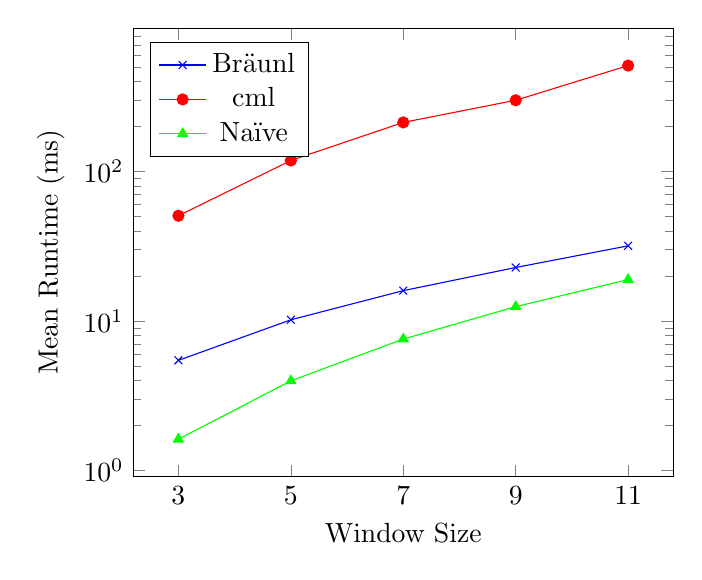
\begin{tikzpicture}
\begin{semilogyaxis}[
	xlabel=Window Size,
    ylabel=Mean Runtime (ms),
    legend pos=north west,
    %xmin=3,
    %xmax=11,
    %minor x tick num=2,
    xtick=data
]
	\addplot [mark=x,blue] table [x=windowSize,y=Mean]{
    	Method	windowSize	filename	Mean	Error	StdDev	Median	Min	Scaled	ScaledSD	Gen0	Gen1	Gen2	Allocated
Bräunl	3	very-small	5.462	0.109	0.285	5.461	4.696	3.37	0.17	31.25	15.625	15.625	2.11
Bräunl	5	very-small	10.195	0.202	0.543	10.087	9.467	2.56	0.14	46.875	31.25	15.625	3.52
Bräunl	7	very-small	15.973	0.318	0.724	15.830	15.012	2.11	0.09	46.875	15.625	-	6.04
Bräunl	9	very-small	22.807	0.447	0.829	22.497	21.855	1.83	0.07	93.75	31.25	-	9.86
Bräunl	11	very-small	31.843	0.621	0.891	31.955	29.750	1.68	0.05	187.5	62.5	-	15.63


    };
    \addplot [mark=*,red] table [x=windowSize,y=Mean]{
    	Method	windowSize	filename	Mean	Error	StdDev	Median	Min	Scaled	ScaledSD	Gen0	Gen1	Gen2	Allocated
\gls{cml}	3	very-small	50.588	2.544	7.500	49.480	40.127	31.18	4.6	166.6667	83.3333	-	1.68
\gls{cml}	5	very-small	118.463	2.349	3.443	119.399	106.345	29.75	0.99	400	200	-	1.69
\gls{cml}	7	very-small	212.817	7.252	21.270	220.862	152.973	28.08	2.79	1000	-	-	1.73
\gls{cml}	9	very-small	299.339	5.264	4.396	298.044	296.011	23.98	0.34	2000	1000	-	1.83
\gls{cml}	11	very-small	510.526	10.065	9.414	510.343	489.584	26.97	0.51	3000	1000	-	1.85

    };
    \addplot [mark=triangle*,green] table [x=windowSize,y=Mean]{
    	Method	windowSize	filename	Mean	Error	StdDev	Median	Min	Scaled	ScaledSD	Gen0	Gen1	Gen2	Allocated
Naïve	3	very-small	1.623	0.003	0.003	1.623	1.618	1	0	154.2969	35.1563	-	2.35
Naïve	5	very-small	3.983	0.076	0.071	3.980	3.891	1	0	382.8125	85.9375	-	5.62
Naïve	7	very-small	7.578	0.011	0.009	7.575	7.566	1	0	734.375	164.0625	-	10.52
Naïve	9	very-small	12.483	0.025	0.022	12.483	12.445	1	0	1171.875	203.125	-	17.26
Naïve	11	very-small	18.933	0.123	0.115	18.896	18.823	1	0	1718.75	187.5	-	23.9
    };
    
    \legend{Bräunl,\gls{cml},Naïve}
\end{semilogyaxis}
\end{tikzpicture}
\caption{\label{graph:median:verysmall}Plot of mean runtimes with a logarithmic y axis for the very small size image}
\end{figure}

%peppers
\begin{figure}
\centering
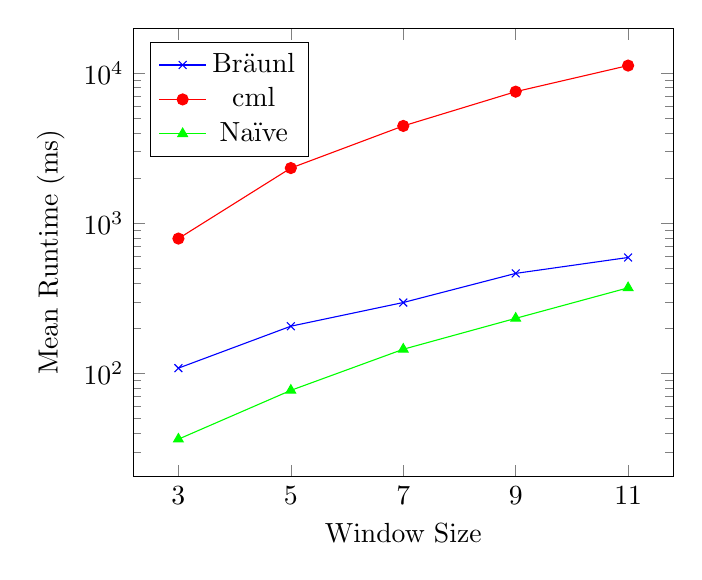
\begin{tikzpicture}
\begin{semilogyaxis}[
	xlabel=Window Size,
    ylabel=Mean Runtime (ms),
    legend pos=north west,
    %xmin=3,
    %xmax=11,
    %minor x tick num=2,
    xtick=data
]
	\addplot [mark=x,blue] table [x=windowSize,y=Mean]{
    	Method	windowSize	filename	Mean	Error	StdDev	Median	Min	Scaled	ScaledSD	Gen0	Gen1	Gen2	Allocated
Bräunl	3	peppers_gray	108.436	2.141	5.088	108.817	93.931	2.98	0.18	1200	1000	1000	37.73
Bräunl	5	peppers_gray	206.336	4.112	9.693	205.430	187.900	2.68	0.15	1000	666.6667	666.6667	58.64
Bräunl	7	peppers_gray	296.717	5.718	5.616	297.432	286.169	2.05	0.12	2000	1000	1000	114.81
Bräunl	9	peppers_gray	463.857	9.138	8.975	464.704	449.199	2	0.13	3000	2000	1000	127.86
Bräunl	11	peppers_gray	592.056	11.749	21.483	589.079	557.281	1.62	0.21	5000	2000	1000	212.34

    };
    \addplot [mark=*,red] table [x=windowSize,y=Mean]{
    	Method	windowSize	filename	Mean	Error	StdDev	Median	Min	Scaled	ScaledSD	Gen0	Gen1	Gen2	Allocated
\gls{cml}	3	peppers_gray	791.285	15.397	23.971	791.190	749.316	21.73	1.09	4000	2000	1000	28.14
\gls{cml}	5	peppers_gray	2333.317	46.639	79.197	2339.807	2108.572	30.29	1.42	8000	3000	2000	28.67
\gls{cml}	7	peppers_gray	4452.903	88.038	183.769	4407.427	4177.586	30.83	2.09	14000	5000	2000	28.28
\gls{cml}	9	peppers_gray	7533.048	150.341	225.023	7527.491	7100.467	32.49	2.2	21000	7000	2000	28.29
\gls{cml}	11	peppers_gray	11237.458	192.938	180.475	11266.773	10925.938	30.74	3.81	32000	10000	4000	29.38
    };
    \addplot [mark=triangle*,green] table [x=windowSize,y=Mean]{
    	Method	windowSize	filename	Mean	Error	StdDev	Median	Min	Scaled	ScaledSD	Gen0	Gen1	Gen2	Allocated
Naïve	3	peppers_gray	36.474	0.724	1.495	36.450	33.341	1	0	3357.1429	1000	1000	36.94
Naïve	5	peppers_gray	77.122	1.532	2.602	77.005	71.833	1	0	7285.7143	1000	1000	87.78
Naïve	7	peppers_gray	144.854	2.895	8.119	142.671	132.158	1	0	13750	1000	1000	175.21
Naïve	9	peppers_gray	232.750	5.198	15.245	227.335	213.438	1	0	21666.6667	1666.6667	1000	239.09
Naïve	11	peppers_gray	371.789	17.122	50.485	345.788	313.159	1	0	32000	1000	1000	337.86
    };
    
    \legend{Bräunl,\gls{cml},Naïve}
\end{semilogyaxis}
\end{tikzpicture}
\caption{\label{graph:median:peppers}Plot of mean runtimes with a logarithmic y axis for the peppers image}
\end{figure}

%small
\begin{figure}
\centering
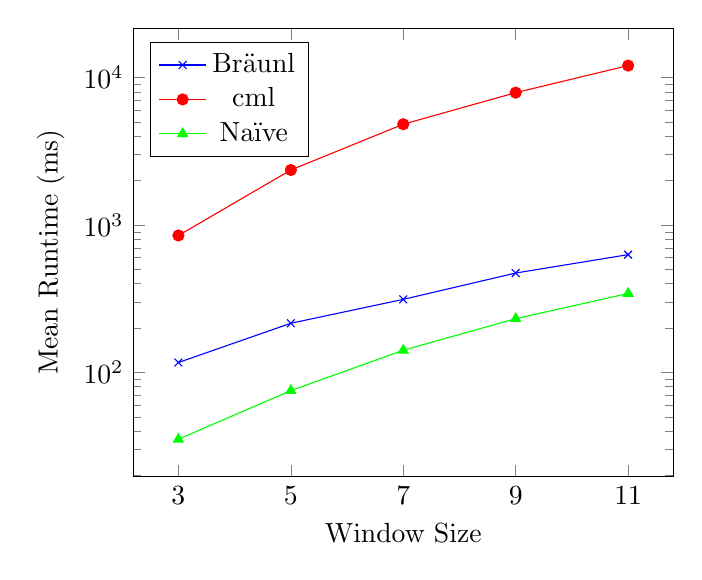
\begin{tikzpicture}
\begin{semilogyaxis}[
	xlabel=Window Size,
    ylabel=Mean Runtime (ms),
    legend pos=north west,
    %xmin=3,
    %xmax=11,
    %minor x tick num=2,
    xtick=data
]
	\addplot [mark=x,blue] table [x=windowSize,y=Mean]{
    	Method	windowSize	filename	Mean	Error	StdDev	Median	Min	Scaled	ScaledSD	Gen0	Gen1	Gen2	Allocated
Bräunl	3	small	116.782	2.334	4.208	116.874	107.437	3.32	0.14	1200	1000	800	40.96
Bräunl	5	small	215.573	4.295	12.185	217.475	180.880	2.86	0.16	1666.6667	1333.3333	1000	63.03
Bräunl	7	small	313.114	2.952	2.761	312.674	309.410	2.21	0.02	2000	1000	1000	111.37
Bräunl	9	small	472.517	4.680	4.378	473.456	460.456	2.04	0.02	4000	2000	1000	161.63
Bräunl	11	small	629.898	5.558	4.927	628.729	618.231	1.83	0.02	5000	2000	1000	149.05

    };
    \addplot [mark=*,red] table [x=windowSize,y=Mean]{
    	Method	windowSize	filename	Mean	Error	StdDev	Median	Min	Scaled	ScaledSD	Gen0	Gen1	Gen2	Allocated
\gls{cml}	3	small	849.482	19.570	56.149	828.209	773.390	24.12	1.69	4000	2000	1000	33.68
\gls{cml}	5	small	2362.643	46.461	104.871	2355.982	2162.910	31.39	1.39	9000	3000	2000	33.25
\gls{cml}	7	small	4830.294	95.856	137.474	4834.632	4523.971	34.15	0.97	14000	5000	2000	33.04
\gls{cml}	9	small	7910.925	134.530	125.839	7909.106	7701.102	34.15	0.54	23000	8000	3000	34.13
\gls{cml}	11	small	12074.170	232.388	228.236	12042.342	11712.425	35.17	0.66	32000	11000	3000	34

    };
    \addplot [mark=triangle*,green] table [x=windowSize,y=Mean]{
    	Method	windowSize	filename	Mean	Error	StdDev	Median	Min	Scaled	ScaledSD	Gen0	Gen1	Gen2	Allocated
Naïve	3	small	35.246	0.697	0.881	34.905	34.267	1	0	3466.6667	1000	1000	37.65
Naïve	5	small	75.282	0.506	0.473	75.217	74.419	1	0	7857.1429	1000	1000	95.36
Naïve	7	small	141.432	0.804	0.752	141.446	140.203	1	0	14000	1000	1000	175.74
Naïve	9	small	231.667	0.979	0.867	232.029	229.561	1	0	22666.6667	1666.6667	1000	328.08
Naïve	11	small	343.286	1.710	1.600	342.643	341.541	1	0	33000	1000	1000	261.29
    };
    
    \legend{Bräunl,\gls{cml},Naïve}
\end{semilogyaxis}
\end{tikzpicture}
\caption{\label{graph:median:small}Plot of mean runtimes with a logarithmic y axis for the small size image}
\end{figure}

%medium
\begin{figure}
\centering
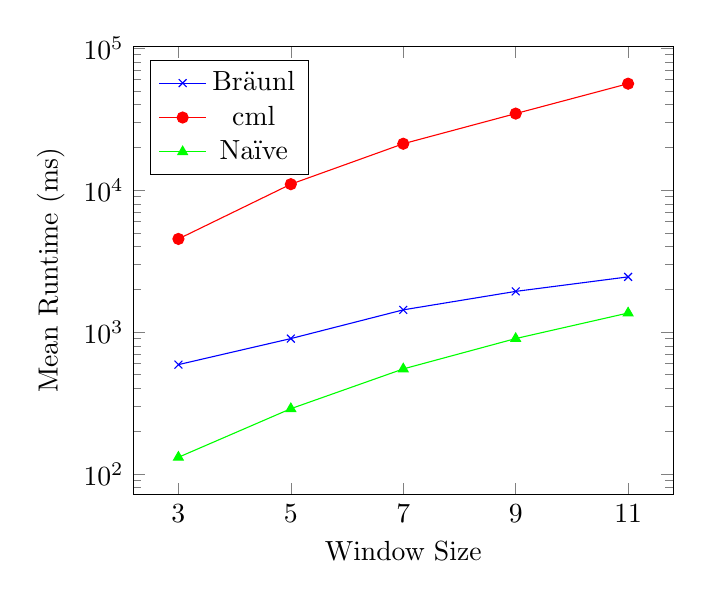
\begin{tikzpicture}
\begin{semilogyaxis}[
	xlabel=Window Size,
    ylabel=Mean Runtime (ms),
    legend pos=north west,
    %xmin=3,
    %xmax=11,
    %minor x tick num=2,
    xtick=data
]
	\addplot [mark=x,blue] table [x=windowSize,y=Mean]{
    	Method	windowSize	filename	Mean	Error	StdDev	Median	Min	Scaled	ScaledSD	Gen0	Gen1	Gen2	Allocated
Bräunl	3	medium	589.431	11.668	10.344	585.135	574.774	4.51	0.27	2000	1000	1000	146.49
Bräunl	5	medium	899.233	4.445	3.940	899.270	892.109	3.12	0.07	4000	2000	1000	230.3
Bräunl	7	medium	1433.220	31.164	29.151	1431.262	1379.761	2.61	0.07	7000	4000	2000	374.04
Bräunl	9	medium	1933.758	24.222	22.657	1925.642	1905.768	2.15	0.02	16000	4000	2000	527.35
Bräunl	11	medium	2447.284	47.271	50.580	2451.473	2352.536	1.8	0.05	40000	4000	2000	167.19

    };
    \addplot [mark=*,red] table [x=windowSize,y=Mean]{
    	Method	windowSize	filename	Mean	Error	StdDev	Median	Min	Scaled	ScaledSD	Gen0	Gen1	Gen2	Allocated
\gls{cml}	3	medium	4527.962	89.754	226.819	4511.961	4003.316	34.65	2.61	12000	6000	3000	132.41
\gls{cml}	5	medium	11006.775	197.445	184.691	10983.829	10737.131	38.19	1.05	28000	10000	4000	138.84
\gls{cml}	7	medium	21210.296	417.303	409.847	21118.240	20410.160	38.61	1.08	50000	15000	4000	136.78
\gls{cml}	9	medium	34587.347	471.655	441.186	34687.611	33898.247	38.45	0.48	81000	22000	4000	137.63
\gls{cml}	11	medium	56196.611	1118.853	2548.193	55158.372	52956.449	41.29	2.05	230000	66000	4000	132.75
    };
    \addplot [mark=triangle*,green] table [x=windowSize,y=Mean]{
    	Method	windowSize	filename	Mean	Error	StdDev	Median	Min	Scaled	ScaledSD	Gen0	Gen1	Gen2	Allocated
Naïve	3	medium	131.111	2.655	7.787	128.188	122.294	1	0	11500	1500	1500	102.34
Naïve	5	medium	288.343	5.716	6.805	285.656	282.623	1	0	28000	1000	1000	371.43
Naïve	7	medium	549.600	12.951	12.114	543.465	539.418	1	0	54000	1000	1000	710.4
Naïve	9	medium	899.563	3.131	2.444	900.523	893.992	1	0	89000	2000	1000	985.29
Naïve	11	medium	1361.629	27.108	31.217	1350.193	1344.088	1	0	131000	4000	1000	1969.78
    };
    
    \legend{Bräunl,\gls{cml},Naïve}
\end{semilogyaxis}
\end{tikzpicture}
\caption{\label{graph:median:medium}Plot of mean runtimes with a logarithmic y axis for the medium size image}
\end{figure}

%\gls{cml}
\begin{figure}
\centering
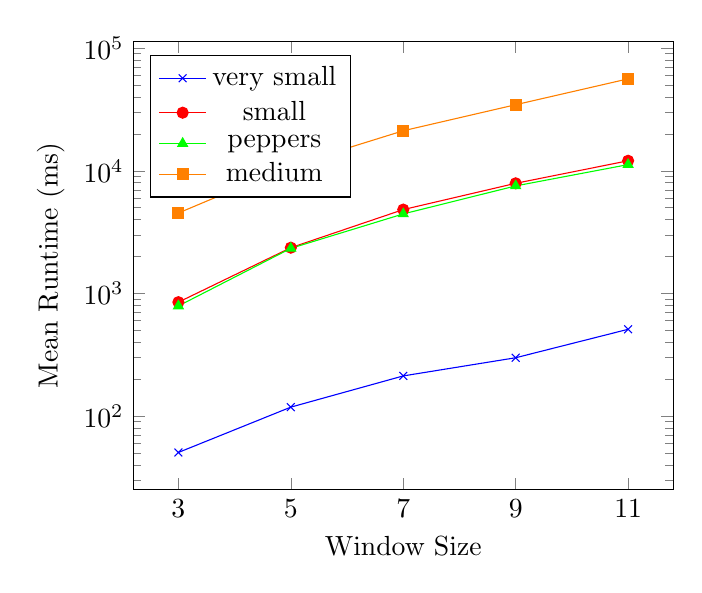
\begin{tikzpicture}
\begin{semilogyaxis}[
	xlabel=Window Size,
    ylabel=Mean Runtime (ms),
    legend pos=north west,
    %xmin=3,
    %xmax=11,
    %minor x tick num=2,
    xtick=data
]
	\addplot [mark=x,blue] table [x=windowSize,y=Mean]{
    	Method	windowSize	filename	Mean	Error	StdDev	Median	Min	Scaled	ScaledSD	Gen0	Gen1	Gen2	Allocated
\gls{cml}	3	very-small	50.588	2.544	7.500	49.480	40.127	31.18	4.6	166.6667	83.3333	-	1.68
\gls{cml}	5	very-small	118.463	2.349	3.443	119.399	106.345	29.75	0.99	400	200	-	1.69
\gls{cml}	7	very-small	212.817	7.252	21.270	220.862	152.973	28.08	2.79	1000	-	-	1.73
\gls{cml}	9	very-small	299.339	5.264	4.396	298.044	296.011	23.98	0.34	2000	1000	-	1.83
\gls{cml}	11	very-small	510.526	10.065	9.414	510.343	489.584	26.97	0.51	3000	1000	-	1.85


    };
    \addplot [mark=*,red] table [x=windowSize,y=Mean]{
    	Method	windowSize	filename	Mean	Error	StdDev	Median	Min	Scaled	ScaledSD	Gen0	Gen1	Gen2	Allocated
\gls{cml}	3	small	849.482	19.570	56.149	828.209	773.390	24.12	1.69	4000	2000	1000	33.68
\gls{cml}	5	small	2362.643	46.461	104.871	2355.982	2162.910	31.39	1.39	9000	3000	2000	33.25
\gls{cml}	7	small	4830.294	95.856	137.474	4834.632	4523.971	34.15	0.97	14000	5000	2000	33.04
\gls{cml}	9	small	7910.925	134.530	125.839	7909.106	7701.102	34.15	0.54	23000	8000	3000	34.13
\gls{cml}	11	small	12074.170	232.388	228.236	12042.342	11712.425	35.17	0.66	32000	11000	3000	34

    };
    \addplot [mark=triangle*,green] table [x=windowSize,y=Mean]{
    	Method	windowSize	filename	Mean	Error	StdDev	Median	Min	Scaled	ScaledSD	Gen0	Gen1	Gen2	Allocated
\gls{cml}	3	peppers_gray	791.285	15.397	23.971	791.190	749.316	21.73	1.09	4000	2000	1000	28.14
\gls{cml}	5	peppers_gray	2333.317	46.639	79.197	2339.807	2108.572	30.29	1.42	8000	3000	2000	28.67
\gls{cml}	7	peppers_gray	4452.903	88.038	183.769	4407.427	4177.586	30.83	2.09	14000	5000	2000	28.28
\gls{cml}	9	peppers_gray	7533.048	150.341	225.023	7527.491	7100.467	32.49	2.2	21000	7000	2000	28.29
\gls{cml}	11	peppers_gray	11237.458	192.938	180.475	11266.773	10925.938	30.74	3.81	32000	10000	4000	29.38
    };
    \addplot [mark=square*,orange] table [x=windowSize,y=Mean]{
    	Method	windowSize	filename	Mean	Error	StdDev	Median	Min	Scaled	ScaledSD	Gen0	Gen1	Gen2	Allocated
\gls{cml}	3	medium	4527.962	89.754	226.819	4511.961	4003.316	34.65	2.61	12000	6000	3000	132.41
\gls{cml}	5	medium	11006.775	197.445	184.691	10983.829	10737.131	38.19	1.05	28000	10000	4000	138.84
\gls{cml}	7	medium	21210.296	417.303	409.847	21118.240	20410.160	38.61	1.08	50000	15000	4000	136.78
\gls{cml}	9	medium	34587.347	471.655	441.186	34687.611	33898.247	38.45	0.48	81000	22000	4000	137.63
\gls{cml}	11	medium	56196.611	1118.853	2548.193	55158.372	52956.449	41.29	2.05	230000	66000	4000	132.75
    };
    
    \legend{very small,small,peppers,medium}
\end{semilogyaxis}
\end{tikzpicture}
\caption[Plot of mean runtimes for the \glsentrylong{cml-glossary} algorithm on different image sizes]{\label{graph:median:cmls}Plot of mean runtimes with a logarithmic y axis for the \gls{cml} algorithm on different image sizes}
\end{figure}

\begin{figure}
\centering
\subcaptionbox{Original}{\includegraphics[width=0.41\textwidth]{chapters/medianfilter/images/peppers/peppers_gray.png}}
\subcaptionbox{Noisy}{\includegraphics[width=0.41\textwidth]{chapters/medianfilter/images/peppers/peppers_gray_noisy.png}}
\subcaptionbox{Naïve}{\includegraphics[width=0.41\textwidth]{chapters/medianfilter/images/peppers/naive_peppers_gray_noisy_3.png}}
\subcaptionbox{Bräunl}{\includegraphics[width=0.41\textwidth]{chapters/medianfilter/images/peppers/braunl_peppers_gray_noisy_3.png}}
\subcaptionbox{\gls{cml}}{\includegraphics[width=0.41\textwidth]{chapters/medianfilter/images/peppers/cml_peppers_gray_noisy_3.png}}
\caption[The classic grayscale `peppers' image, before and after processing]{\label{fig:median:peppers}The classic greyscale `peppers' image, before and after processing.  (a) is the original image; (b) is the image with random salt \& pepper noise introduced; (c) is the result of processing the image using the naïve algorithm; (d) is the result of processing the image using the Br\"{a}unl-inspired algorithm; (e) is the result of processing the image using the \gls{cml} algorithm}
\end{figure}

\begin{table}
\centering
\caption[Peak signal-to-noise for the very small image]{Peak signal-to-noise ratio for the very small image (measured in decibels)}
\label{tab:median:psnrvsmall}
\begin{tabular}{@{}lccccc@{}}
\toprule
\multicolumn{1}{c}{\textbf{Algorithm}} & \multicolumn{5}{c}{\textbf{Window size}}                                          \\
                                       & 3              & 5              & 7              & 9             & 11             \\ \midrule
Bräunl                                 & 20.78          & 17.82          & 15.65          & 14.36         & 13.55          \\
\gls{cml}                                    & 25.98          & \textbf{21.85} & \textbf{18.62} & \textbf{16.40} & 14.99          \\
Naïve                                  & \textbf{27.03} & 21.74          & 18.55          & 16.39         & \textbf{15.02} \\ \bottomrule
\end{tabular}
\end{table}

\begin{table}
\centering
\caption[Peak signal-to-noise for the peppers image]{Peak signal-to-noise ratio for the peppers image (measured in decibels)}
\begin{tabular}{@{}lccccc@{}}
\toprule
\multicolumn{1}{c}{\textbf{Algorithm}} & \multicolumn{5}{c}{\textbf{Window size}}                                          \\
                                       & 3              & 5              & 7              & 9              & 11            \\ \midrule
Bräunl                                 & 28.76          & 27.35          & 25.27          & 23.94          & 22.82         \\
\gls{cml}                                    & 31.85          & 31.07          & 29.8           & 28.56          & 27.42         \\
Naïve                                  & \textbf{32.79} & \textbf{31.25} & \textbf{29.87} & \textbf{28.63} & \textbf{27.50} \\ \bottomrule
\end{tabular}
\label{tab:median:psnrpeppers}
\end{table}

\begin{table}
\centering
\caption[Peak signal-to-noise for the small image]{Peak signal-to-noise ratio for the small image (measured in decibels)}
\label{tab:median:psnrsmall}
\begin{tabular}{@{}lccccc@{}}
\toprule
\multicolumn{1}{c}{\textbf{Algorithm}} & \multicolumn{5}{c}{\textbf{Window size}}                                          \\
                                       & 3              & 5              & 7             & 9              & 11             \\ \midrule
Bräunl                                 & 32.83          & 32.34          & 30.74         & 29.73          & 28.94          \\
\gls{cml}                                    & 36.62          & 34.25          & 32.66         & 31.57          & 30.71          \\
Naïve                                  & \textbf{37.83} & \textbf{34.31} & \textbf{32.7} & \textbf{31.65} & \textbf{30.81} \\ \bottomrule
\end{tabular}
\end{table}

\begin{table}
\centering
\caption[Peak signal-to-noise for the medium image]{Peak signal-to-noise ratio for the medium image (measured in decibels)}
\begin{tabular}{@{}lccccc@{}}
\toprule
\multicolumn{1}{c}{\textbf{Algorithm}} & \multicolumn{5}{c}{\textbf{Window size}}                                           \\
                                       & 3              & 5              & 7              & 9              & 11             \\ \midrule
Bräunl                                 & 32.98          & 32.65          & 31.59          & 30.91          & 30.36          \\
\gls{cml}                                    & 36.72          & \textbf{34.15} & \textbf{32.98} & \textbf{32.26} & \textbf{31.73} \\
Naïve                                  & \textbf{37.16} & 34.07          & 32.96          & \textbf{32.26} & \textbf{31.73} \\ \bottomrule
\end{tabular}
\label{tab:median:psnrmedium}
\end{table}

Examination of the reported memory statistics (please see the GitHub repository for details) appears to show that the maximum amount of memory allocated during processing for the \gls{cml} algorithm stays roughly constant across window sizes for each image size, and in fact on larger window sizes it is the most memory efficient.  The naïve algorithm quickly grows to consume the most memory at larger window sizes for each image size, suggesting that it likely derives some of its comparative speed at the cost of greater space complexity, while Bräunl sits in the middle.  Conversely, \gls{cml} generates by far the most garbage collection events, which may help explain its relative sluggishness.

\section{Discussion}

The algorithms developed and presented here are not necessarily optimal for the purpose.  They largely handle each pixel separately, or combine them into arrays on-the-fly.  This ignores the possibility of exploiting data-parallelism to improve throughput, and instead relies only on the separate CPU cores to provide parallelism.

It is unclear how much the mechanics underlying these implementations (\ie{} the .NET Core and \hopac{} systems) attempt to maximise use of the processor cache.  Efficient use of the cache can contribute significantly to an optimised version of an algorithm outperforming, a simplistic version by an order of magnitude or more \cite{Ragan-Kelley2017}.  No attempt was made manually to ensure good practices, such as tiling or striping \cite{Midkiff2012}.

The \gls{cml} approach used in essence instantiates a \gls{pe} for each pixel, each of which must be scheduled to run at some point --- concurrent with another \gls{pe} in the case of synchronous message passing.  It is possible that this surfeit of separate logical threads may induce excessive switching costs, and perhaps promote wasted time, with threads regularly polling their channel and their neighbours'.  Careful improvements to this and the use of the cache might lead to significant gains in speed.

In terms of the code itself also, \gls{cml} appears to be the worst.  The program requires roughly double the number of lines of the naïve program, and is arguably much less `clean' or `readable'.  Reinterpreting the \gls{medianfilter} in terms of \glsxtrlong{csp} has not yielded a structural improvement nor simplified the programming task.  Combined with the running time results above, this suggests that the \gls{cml} approach is actively counter-productive for implementing \glspl{mwt}, at least when using \hopac{}.

Basic profiling of the \gls{cml}-based implementation appears to show that more than half of the runtime of the program was spent inside the function for giving a value over a channel, and functions called by it.  Furthermore, according to this profiling, almost 40\% of the total running time of the algorithm is taken up specifically by low-level memory management functions inside the depths of the .NET Core system.  Considering that some of these functions \fxwarning{ref?}{are written in hand-optimised assembly}, the fact they account for so much of the running time appears to suggest that memory use is poorly handled in the tested implementation.

\Glspl{mwt} are generally relatively simplistic processes, typically consisting simply of combining values from the pixel array, and which can be programmed in a straightforward fashion.  More sophisticated programming techniques may simply `get in the way' and introduce unnecessary overheads, which appears to have happened here.  Furthermore, the \gls{medianfilter} can largely be broken down into arithmetic and logical operations amenable to vectorisation (\eg{} \cite{Sanchez2012,Perreault2007}), which the \gls{cml} approach currently ignores entirely.

% \subsection{Threats to validity}
\subsection{Experimental Limitations}
There are two identifiable threats to validity, both regarding the `quality' of the programming involved.  .NET Core, as a widely used open-source compiler and runtime system, and which has likely had millions of man-hours invested in it, is presumably of high quality and fast in most cases.  That is not necessarily the case with \hopac{}.  While it is open source, and moderately well-known in the \fsharp{} community, the amount of time spent on optimising it is likely nowhere close to that spent on .NET Core.  Consequently, \hopac{} itself may present significant bottlenecks while performing the \gls{mwt}.

The other threat to validity (as with all performance-focused experiments) is the skill of the end programmer.  The author was new to the \hopac{} library at the start of this work, and inferior design choices may have been made unwittingly.  It was, however, suggested during personal communication with one of the maintainers and fellow users of the \hopac{} library that the \gls{cml} approach may simply be a poor fit to pixel-wise image processing tasks.

Fundamentally, the results achieved here, as with most implementation exercises, succeed or fail in large part on the skill, knowledge and effort of the programmers involved.  The use of other libraries may lead to better results.  Other parallel implementations of \gls{cml} exist, such as Concurrent Haskell \cite{Chaudhuri2009}, Manticore \cite{Reppy2009a} and Fibers\footnote{\url{https://github.com/wingo/fibers}} for Guile Scheme, but have not been assessed for this work.

\section{Summary}

Motivated by an interest in representing the \gls{medianfilter} process in \gls{cps}, this \namecref{chap:median} considered the implementation of common statistical operations over natural numbers in \gls{cps}, using \gls{cps}' typical representation of natural numbers via unary arithmetic.  In particular, the following groups of operations on (multi)sets were demonstrated:
\begin{inparaenum}[(i)]
\item Choosing the minimum and maximum elements;
\item Determining the magnitude of a (multi)set, and frequency of occurrence of each element within;
\item Computing the sum, mean, and mode over the elements;
\item Sorting the elements numerically (along with necessary extra structure to make the sorting meaningful);
\item Selecting the \(n^\text{th}\) element of a (multi)set, and thus also determining the median.
\end{inparaenum}

Most of the operations work identically for both sets and multisets.  In cases where they don't, the difference arises because of meaningful differences in the nature of sets and multisets.  Furthermore, \emph{all} of these operations work in constant time regardless of input size, and all require a fixed number of rules per operation.  These operations also compose well.  Indeed, the operations to compute the mean, mode, and median of a multiset are all formed out of other operations described herein.  Notably, all but the operations to select a minimum and maximum use at least one \gls{ms} in their ruleset.

Each operation was presented alongside a table providing an example evolution of a system with a specific (multi)set as input.  Furthermore, a sample system to perform image \gls{medianfilter}ing, plus application of it to an example image were provided in \cref{sec:median:cpsmedianfilter,sec:median:cpsmedianexample}.  The choice of image \gls{medianfilter}ing was motivated by two main factors:
\begin{inparaenum}[(i)]
\item the embarrassingly parallel nature of many image processing operations;
\item the clear opportunity to provide a concrete example of the inter-\gls{tlc} communications described in \cref{sec:cps:intertlcmess} and demonstrate further the capabilities of \gls{cps} in implementing a simple but non-trivial image processing task.
\end{inparaenum}
As with the systems in \cref{chap:tsp,chap:gcol}, so long as the system has been correctly configured with one \gls{tlc} per image pixel, and each \gls{tlc} knows its neighbours, the entire process requires only one fixed ruleset regardless of the specific image to be filtered.

The use of a \gls{cml} approach to image processing was explored in this \namecref{chap:median}, in particular as applied to the \gls{medianfilter} \gls{mwt} operation.  The design of the \glspl{cps}, with its heavy use of communication, points naturally to the use of \gls{cml} for a simulation.  The measured results suggest that it is much worse than using a simple, naïve nested \texttt{for loop}s approach.  The reason for this appears to be related primarily to overhead from the synchronous communications, especially memory allocations and garbage collections.  This may be an issue with the \gls{cml} style in general, or it may be an issue related to the \gls{cml} library used or the programming of the algorithms tested here.  More work is required to determine this for certain.  \Gls{cml} does appear to provide one advantage, however, in that with larger window sizes, it seemingly has the lowest peak space requirement.

A \gls{cml} approach where a separate \glsxtrlong{pe} is used to represent each pixel largely eliminates the possibility of taking advantage of data-parallel hardware, such as \glspl{gpu} or vector instructions of CPUs.  For situations where vector instructions are applicable, the \gls{cml} approach seems likely to be a poor choice.  It is not clear, however, how well this approach may or may not work for instances where the data types involved are more complex, or where there is a significant level of control flow involved.  Nor has there been any investigation so far into the practicality of assigning multiple pixels to a single \glsxtrlong{pe}.